\typeout{NT FILE evaluation.tex}%

\glsresetall
\chapter{Evaluation}

% In this section we evaluate Marrow-Graph from the correctness, expressiveness and performance
% perspectives. To this end, we compare Marrow-Graph against a set of state-of-the-art graph processing frameworks.

In this section, we evaluate Marrow-Graph against a set of state-of-the-art graph processing frameworks. The main goals of this evaluation are
\begin{enumerate*}
    \item Verifying the correctness of Marrow-Graph's operations and algorithms.
    \item Assessing Marrow-Graph's expressiveness and simplicity.
    \item Evaluating Marrow-Graph's performance.
\end{enumerate*}

\section{Correctness}

To verify the correctness of Marrow-Graph, we try to answer the following questions:
\begin{itemize}
    \item Do all graph mutation operations result in the expected graph state?
    \item Do all the traversal operators output the expected result?
    \item Do all of Marrow-Graph's algorithms output the expected result?
\end{itemize}

To this end, multiple unit tests (using Google Test) were developed during Marrow-Graph's development. Additionally, we compare Marrow-Graph's algorithmic outputs with Gunrock's. The developed unit tests include:
\begin{enumerate*}
    \item Testing the advance and filter operators for both small/trivial examples, and using large graphs and complex compute and segmented intersection operators.
    \item Testing all the graph mutation functions.
    \item Testing the loading of large batches of edge and vertex insertions and deletions and ensuring a correct final state.
\end{enumerate*}

To ensure the correctness of the developed algorithms, we executed all the algorithms on Marrow-Graph and Gunrock, using real-life-large graphs, namely RoadNet-CA (Table~\ref{tab:graph_stats}) and hollywood-2009 (Table~\ref{tab:graph_stats}), and compared their respective outputs. For \gls{BFS}, \gls{SSSP}, and \gls{TC}, we were able to achieve the exact same output results as Gunrock.  \gls{PR} deals with many floating point operations, for this reason, very similar output results were obtained, but with some small deviations. To ensure that the deviations were indeed just related to floating-point rounding issues, we compared all the outputted elements and ensured that their absolute differences were bellow \texttt{FLT\_EPSILON}. \texttt{FLT\_EPSILON} is a commonly used floating-point value to access floating-point similarity. Its defined by the standard library as the "difference between 1 and the least value greater than 1 that is representable"~\cite{cppreference}. For \gls{SpMV} we were able to achieve very similar results, but again with slight deviations. We were not able to achieve an output result with absolute differences smaller than \texttt{FLT\_EPSILON} for \gls{SpMV}. The exact cause for this has not been completely determined, but might also be related to floating point rounding errors.

We can conclude that Marrow-Graph's manipulation functions and operators are indeed following the expected behavior, and that all the algorithms are outputting mostly identical results to the current state-of-the-art \gls{GPU}-accelerated graph processing framework. 

% We can conclude that Marrow-Graph is indeed operating correctly, and outputing similar algorithmic results, as the current state-of-the-art \gls{GPU}-accelerated graph processing framework. 

\section{Expressiveness and Simplicity}
\label{sec:evaluation_expressiveness}

To access the expressiveness and simplicity of Marrow-Graph, we try to answer the following questions:
\begin{itemize}
    \item Can Marrow-Graph express most graph-analytics algorithms?
    \item Can algorithms and programs be expressed in Marrow-Graph in a simple and concise manner?
\end{itemize}

\subsection{Evaluation Methodology}

For this evaluation, we compare the implementations of a set of common graph algorithms against Gunrock, FaimGraph, and Hornet. As metrics to answer the previous questions, we will consider:

\begin{description}
    \item \textbf{Implementable Algorithms}: Number of common algorithms that have been implemented, or can theoretically be implemented.
    \item \textbf{Conciseness}: How much code and boilerplate is required to express an algorithm.
    \item \textbf{Readability}: How readable or obfuscated the implementations of algorithms are.
\end{description}

For the first, we will compare the total set of implemented algorithms by each framework. For the second, we will compare the total number of useful lines of code that comprise each framework's implementation. When we refer to useful lines of code, this means discarding any empty lines, comments, and code unrelated to the algorithm (for example debug logs and validation functions). For readability, we will directly compare some of the implementation details and syntax of each framework.

\subsection{Results}

Regarding expressiveness, Table~\ref{tab:graph_algorithms} contains a list of common graph algorithms and the frameworks that implement them. As we can see, Gunrock is currently the framework that supports the largest number of algorithms. Implementing 12 of the 15 algorithms considered. Hornet and FaimGraph implement 9 and 7 respectively, supporting some algorithms that are not supported by Gunrock, such as Clustering Coefficient, Connected Components, and others. Marrow-Graph can potentially implement at least 10 algorithms. Because of time constraints, only 5 have indeed been implemented. However, taking into account that Marrow-Graph and Gunrock share a very similar programming model, looking at Gunrock's implementations of these algorithms, we can safely assume that the Betweenness Centrality, Graph Coloring, Geolocation, Hyperlink-Induced Topic Search, and K-Core Decomposition algorithms can theoretically also be implemented in Marrow-Graph. All of these algorithms are implemented using operations that are supported by either Marrow-Graph or marrow. The only algorithm whose implement-ability in Marrow-Graph is uncertain is Minimum Spanning Tree, as it uses a specialized Gunrock operator \texttt{parallal\_for\_each\_t::element}. Additionally, the Local Graph Clustering algorithm is no longer available in the public Gunrock repository. Regarding the algorithms implemented in Hornet and FaimGraph, but not in Gunrock, it is difficult to confidently say whether or not these algorithms are easily implementable in Marrow-Graph. Given their differences in programming models, a more in-depth analysis of these algorithms would be necessary. Regardless, we can conclude that Marrow-Graph already shows a very high level of expressiveness. 
% \todo[inline]{TODO: why are LGC and MSP not imp. MSP -> uses operators::parallel_for_each_t::element which hasn't been studied | LGC -> no longer in repo}

\begin{table}[t]
    \centering
    \small
    \begin{tabular}{|c|c|c|c|c|c|}
        \hline
        Algorithm & Gunrock & Hornet & FaimGraph & Marrow-Graph\\
        \hline
        \hline
        
        Betweeness Centrality & \checkmark & \checkmark & \checkmark & imp.  \\
        Breadth-First Search & \checkmark & \checkmark & \checkmark & \checkmark \\
        Clustering Coefficient & & \checkmark & \checkmark &   \\
        Connected Components & & \checkmark & \checkmark &  \\
        Graph Coloring & \checkmark & &  & imp. \\
        Geolocation & \checkmark & & & imp. \\
        Hyperlink-Induced Topic Search & \checkmark & & & imp. \\
        Katz Centrality & & \checkmark &  & \\
        K-Core Decomposition & \checkmark  & &  & imp. \\
        Minimum Spanning Tree  & \checkmark & &  & \\
        PageRank & \checkmark & \checkmark & \checkmark & \checkmark \\
        Local Graph Clustering & \checkmark & & & \\
        Sparse-Matrix Vector Multiplication & \checkmark & \checkmark & \checkmark & \checkmark \\
        Single-Source Shortest Path & \checkmark & \checkmark & & \checkmark \\
        Triangle Counting & \checkmark & \checkmark & \checkmark & \checkmark  \\
        \hline
    \end{tabular}
    \caption{Implemented graph algorithms (imp: implementable).}
    \label{tab:graph_algorithms}
\end{table}


\begin{table}[t]
    \centering
    \small
    \begin{tabular}{|c|c|c|c|c|}
        \hline
        Algorithm & Gunrock & Hornet & FaimGraph & Marrow-Graph \\
        \hline
        \hline
        
        Breadth-First Search  & 104  & 64 & 68 & 44 \\
        PageRank  & 150 & 73 & 134 & 79 \\
        Sparse-Matrix Vector Multiplication & 116 & 38 & 59 & 18 \\
        Single-Source Shortest Path & 125 & 48 & - & 55 \\
        Triangle Counting & 129 & 95 & 106 & 40 \\
        \hline
    \end{tabular}
    \caption{Number of lines of code composing graph algorithms.}
    \label{tab:lines_graph_algorithms}
\end{table}

Regarding conciseness, we believe that we provide the solution with the most concise, and yet readable, algorithm implementations. While line count is not an entirely objective measure of conciseness, it offers valuable insights. To support our claim, Table \ref{tab:lines_graph_algorithms} displays the total number of useful lines in each framework's implementations of the common algorithms. We can immediately see that Marrow-Graph requires significantly less lines of code than Gunrock and FaimGraph, and slightly less lines of code than Hornet. Marrow-graph only shows a very slightly higher number of lines of code than Hornet in 2 algorithms (\gls{PR} and \gls{SSSP}). In general, Marrow-Graph requires almost no boilerplate code to express these algorithms. Gunrock require a significant amount of boilerplate code, and Hornet algorithms must be defined inside inheriting classes, which require overriding a set of common methods. FaimGraph does not provide a high-level programming model like the other solutions, requiring a more verbose and low-level implementation of the various algorithms.

Besides conciseness, we also believe that we offer the best readability. Although the implementations between Marrow-Graph and Gunrock share many similarities, as already stated, Gunrock requires dealing with a significant amount of boilerplate, but also with a lot of Gunrock-specific concepts, such as contexts, enactors, load-balancing-methods, execution policies, and more. All of these concepts of course allow for more flexibility and control over these algorithms, but also make them less readable, in the sense that the actual algorithm logic becomes more obfuscated. Additionally, Gunrock makes heavy usage of the thrust library, while Marrow-Graph uses marrow. We believe marrow offers a more concise and simpler syntax supported by the adoption of a unified address space, which does not require the programmer to worry about host-device communication and synchronization. One notable superiority of Gunrock over Marrow-Graph lies in its utilization of \texttt{std::function}s and lambdas, which undergo rigorous type-checking. This contrasts with Marrow-Graph's reliance on templated functors, potentially resulting in less transparent compilation errors. Hornet in general also offers algorithms with a good level of readability. Most of the code is directly related to the algorithm's logic, and a set of high-level operators, such as \texttt{forAllEdges} and \texttt{foraAllVertices}, are provided to easy development. Hornet makes use both of functors and lambdas to express operations. Similarly to Gunrock, Hornet has the disadvantage of leaving most device memory management (of problem data) to the programmer using operators such as \texttt{host::copyToDevice}, \texttt{gpu::allocate}, and \texttt{gpu::free}. FaimGraph's main focus is to provide a novel efficient dynamic-graph data structure~\cite{paper:faimgraph}. For this reason, as already stated, it does not include a high-level programming model that allows for simple and accessible algorithm implementations.

\subsection{Conclusion}

From our analysis, we can conclude that Marrow-Graph already demonstrates a high level of expressiveness, and allows for the development of concise and very readable algorithms. 
The integration of a simple, yet powerful interface inspired by Gunrock, with the expressive and user-friendly marrow library, results in a cohesive library that maintains ease of use but also achieves an expressive capability comparable to Gunrock.



\section{Performance}

To assess Marrow-Graph's performance, we will try to answer the following questions
\begin{itemize}
    \item Is there an optimal block size for marrow-graph?
    \item Does Marrow-Graph offer competitive algorithmic and mutative performance against the state-of-the-art \gls{GPU}-accelerated graph processing frameworks?
    \item How does Marrow-Graph's \gls{GPU} usage compare to the state-of-the-art \gls{GPU}-accelerated graph processing frameworks?
\end{itemize}

\subsection{Evaluation Methodology}

For this evaluation, as a baseline, we will use Gunrock~\cite{paper:gunrock}, the state-of-the-art static GPU-Accelerated graph framework, and Ligra~\cite{paper:ligra}, the state-of-the-art static CPU-based graph framework. As our main competitors we will consider Hornet~\cite{paper:hornet} and FaimGraph~\cite{paper:faimgraph}, as these are the current state-of-the-art GPU-Accelerated dynamic graph frameworks.
%
As metrics to answer the previous questions, we will consider: 
\begin{description}
    \item \textbf{Graph initialization time}: Time it takes to load a graph from a file and store it on the device.
    \item \textbf{Graph update rates}: Number of edges/vertices that can be updated per time unit.
    \item \textbf{Algorithmic Time}: Time it takes to execute an algorithm over a graph after it has been loaded and initialized.
    \item \textbf{\gls{GPU} percentile usage}: The amount of processing power that is being consumed by a graph processing application on the \gls{GPU}.
    \item \textbf{\gls{VRAM} Usage}: The amount of \gls{VRAM} that is being consumed by a graph processing application on the \gls{GPU}.
\end{description}

\paragraph{\textbf{Optimal Block-Size}.} In order to determine the optimal block size for Marrow-Graph, we developed a benchmark that measures both graph initialization time, edge insertion time, and algorithmic time, using different block sizes. This benchmark performs a fixed-sized number of small/medium batch insertions, followed by a set of iterations of the \gls{SSSP} algorithm. We chose the \gls{SSSP} algorithm given that it is a fairly complex algorithm that requires multiple iterations, and uses most of Marrow-Graph's functionalities.

\paragraph{\textbf{Graph Initialization}.} In order to measure graph initialization times, we measure the time it takes to load the \texttt{mtx} or \texttt{pbbs} file into memory and upload the constructed graph to the device. All the frameworks use the \texttt{mtx} file format to load the graphs, with the exception of Ligra which uses \texttt{pbbs}.

\paragraph{\textbf{Graph Updates}.} In order to measure update rates, we developed a set of benchmarks that measure the time it takes for a set of update bathes to be loaded into the graph. Both Hornet and FaimGraph allow batches of any size to be loaded onto the graph. We could simply measure the update rates of single large batch insertions using the different frameworks. But in a real-case scenario, updates of different sizes can arrive dynamically. 
% in a non-deterministic manner. 
For this reason, instead of only measuring the optimal case of inserting single large batches of size $N$, we measure the update rates obtained while performing $N$ update operations using multiple batches of varying sizes. Another reason such measurements are more useful is related to the manner in which Marrow-Graph performs its graph updates. Contrary to FaimGraph and Hornet, Marrow-Graph performs updates on the host and synchronizes them to the device whenever an algorithm or operator is executed. This means Marrow-Graph can handle real-time updates of small to medium sizes very efficiently on the host. FaimGraph and Hornet, on the other hand, perform updates directly on the device, meaning that they benefit from using single large batches. In order to fairly portray both the benefits and shortcomings of both methods of performing updates, we measure the update rates using both single large batches, and multiple smaller batches. Ideally, we would like to measure edge and vertex insertion and deletion rates. However, given that Hornet does not directly support vertex updates and that we were not able to perform edge deletions in either framework (runtime errors were always encountered), we only measure edge insertion rates.

\paragraph{\textbf{Algorithms}.}
For algorithmic performance, we will run a set of common graph analytics algorithms, namely: \gls{BFS}, \gls{SSSP}, \gls{TC}, \gls{SpMV} and \gls{PR}. Most of the frameworks implement all of these algorithms, with the exception of FaimGraph which does not implement \gls{SSSP}, and Ligra wich does not implement \gls{SpMV}. However, we did not consider all of the implementations for our benchmarks. FaimGraph's \gls{PR} implementation is different from Marrow-Graph's, Hornet's and Gunrock's, as it uses a fixed size number of iterations, rather than a metric based on the absolute differences between the results of the last two iterations. Additionally, FaimGraph's \gls{SpMV} and Hornet's \gls{TC} both resulted in runtime errors when we tried to run them. In order to achieve fair and comparable results between the frameworks, some small modifications were performed to some of the algorithms, namely:
\begin{itemize}
    \item Ligra's \gls{PR} was modified to use the same alpha and tolerance values as Marrow-Graph.
    \item Hornet's \gls{PR} was modified to use the same alpha and tolerance values as Marrow-Graph, its reduction was changed to use \texttt{max} instead of \texttt{add} (like Marrow-Graph and Gunrock), and an iteration counter was incorporate that could be queried by the benchmark suite. % Additionally, Hornet's build files were edited to fix compilation issues,
    \item Gunrock's \gls{PR} was modified to use the same alpha and tolerance values as Marrow-Graph and an iteration counter was incorporated that could be queried by the benchmark suite.
    \item FaimGraph's \gls{SpMV} was edited to use the non-warped-sized implementation given that the warped-sized implementation resulted in runtime errors.
\end{itemize}

The \gls{PR} algorithm loops until a given condition is met (the tolerance and alpha values we used were $1.0*10^{-6}$ and $0.85$ respectively). To ensure a fair comparison between the different frameworks, we logged the number of iterations performed by each implementation and ensured that they were the same. The other algorithms either don't require iterating (\gls{SpMV} and \gls{TC}), or have a deterministic number of iterations that is not tied to a heuristic (\gls{BFS} and \gls{SSSP}). For all the algorithms that require an initial source vertex, we used the source vertex with ID $0$.

It is worth noting that from the list of algorithms that we chose to use in this benchmark, only \gls{PR} has been implemented by Hornet using the dynamic data structure. Unfortunately, we were not able to use it as it often resulted in runtime errors. This means that all of Hornet's results are not fairly comparable to Marrow-Graph and FaimGraph, as all the algorithms run on the static version.
    
\paragraph{\textbf{Updates + Algorithms}.} Besides measuring algorithmic and mutative performance separately, we also developed a set of benchmarks that measure the performance of doing both operations interchangeably. This means that we load a graph to the device, and then perform $N$ iterations, where we load a single update batch and execute the \gls{SpMV} algorithm in each iteration. We chose \gls{SpMV} because it was the algorithm that displayed the most similar performance across all implementations. Besides Marrow-Graph and FaimGraph, we also included Gunrock in these benchmarks. Although Gunrock does not support graph mutations, we developed a function that emulates the workload of reloading an updated graph. We do so by re-uploading the whole graph from the host to the device. This is somewhat of a conservative approach, given that updating the graph would require reconstructing the CSR data structure before re-uploading it. Regardless, we can still obtain a rough estimation of the performance gains of using dynamic graph frameworks versus static graph frameworks, such as Gunrock, when dealing with both algorithms an mutations. We were not able to include Hornet in this benchmark, given that very few algorithms have been implemented in Hornet using the dynamic data structure (most algorithms only run on the static version), and the few that were, often result in runtime errors.

\paragraph{\textbf{\gls{GPU} Usage}.} In order to compare the \gls{GPU} usage of the different frameworks, we measured the total \gls{GPU} percentile usage, and \gls{VRAM} usage, during the execution of the \texttt{update\_spmv} benchmark. These measurements were performed using the Nvidia-smi tool, with a sampling frequency of 100Hz, or every 10 milliseconds. We chose the \texttt{update\_spmv} benchmark given that it is the most complex and complete benchmark that deals with both graph initialization, graph updates, and algorithm execution.

\paragraph{\textbf{Experimental Setup}.}
%
For our benchmarks, we utilized a subset of the real-life-large-graphs proposed by Gunrock, which are available at the Network Repository~\cite{site:graph_rep}. Some of the larger graphs weren't utilized given the limited \gls{VRAM} of one of the machines used for the execution of the benchmarks. The graph's relevant statistics can be found in Table~\ref{tab:graph_stats}.


\begin{table}
    \centering
    \small
    \begin{tabular}{|c|c|c|c|c|c|}
        \hline
        Name & N. Vertices & N. Edges & Min. Deg. & Max. Deg. & Avg. Deg. \\
        \hline
        \hline
        roadNet-CA & 1.9M & 2.7M & 1 & 12 & 2 \\
        belgium\_osm & 1.4M & 1.5M  & 1 & 10 & 1 \\
        delaunay\_n21 & 2.1M & 6.3M  & 3 & 23 & 5 \\
        hollywood-2009 & 1.1M & 57.5M  & 1 & 11.5K & 105 \\
        road\_usa & 23.9M & 28.9M  & 1 & 9 & 2 \\
        \hline
    \end{tabular}
    \caption{Graph statistics.}
    \label{tab:graph_stats}
\end{table}

All time measurements were conducted utilizing the standard C++ chrono library for accuracy (in the microseconds range) and consistency. To ensure robustness, each algorithm underwent ten iterations, with the average execution time serving as the basis for our results. Regarding compilation, all frameworks use the GCC and NVCC compilers. Additionally, similarly to most of the other frameworks, all Marrow-Graph benchmarks were compiled using the -O3 flag. All benchmarks were executed on the machines detailed in Table~\ref{tab:machines}.

\begin{table}
    \centering
    \small
        \begin{tabular}{|l|l|l|}
            \hline
            & \textbf{Machine 1} & \textbf{Machine 2} \\
            \hline
            \hline
            CPU & Intel Core i5-3570 @ 3.40GHz & AMD Ryzen 5 3600 @ 3.60GHz \\
            GPU & NVIDIA GTX 980 4GB & NVIDIA RTX 3060 12GB \\
            RAM & 8GB DDR3 @ 1600MHz & 16GB DDR4 @ 3200MHz\\
            OS & Ubuntu 22.04.3 LTS & Ubuntu 22.04.3 LTS \\
            Linux kernel & 6.5.0-21 & 6.5.0-14 \\
            NVIDIA driver & 535.154.05 & 545.23.08 \\
            CUDA  & 12.0 & 12.3 \\
            G++   &  11.4.0 & 11.4.0 \\
            \hline
        \end{tabular}
    \caption{Experimental setups.}
    \label{tab:machines}
\end{table}



\subsection{Results}

\paragraph{\textbf{Optimal Block-Size}.} Regarding optimal block-size, we measured the graph load time (Figure~\ref{fig:block_size_graph_load}), edge insertion time (Figure~\ref{fig:block_size_edge_insertion}) and \gls{SSSP} average time (Figure~\ref{fig:block_size_edge_sssp}) using block sizes of 2, 4, 8, 16, 32, 64 and 128. These plots contain the results obtained on Machine 1. Note that the displayed graph load times for the hollywood-2009 graph have all been divided by 10 for improved readability.

\begin{figure}
    \centering
    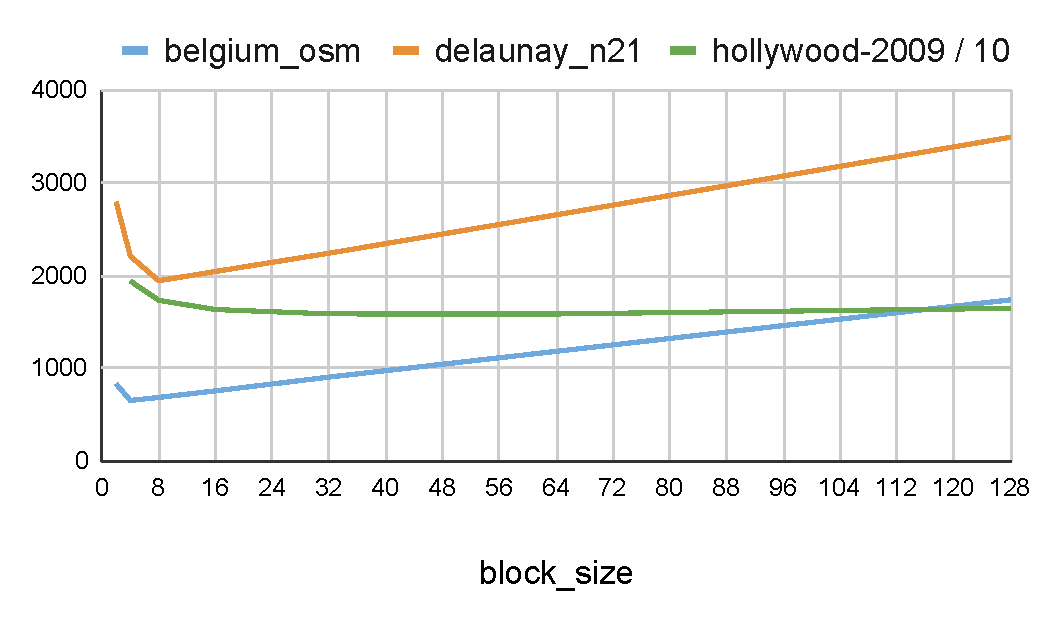
\includegraphics[width=0.7\textwidth]{Chapters/Figures/plots/block_size_graph_load.pdf}
    \caption{Block size benchmark: Total graph load time in milliseconds.}
    \label{fig:block_size_graph_load}
\end{figure}

As we can see in Figure~\ref{fig:block_size_graph_load}, the time it takes to build and upload both the belgium\_osm and delaunay\_n21 graphs, with block-sizes larger than 4, increases linearly with the increase in block size. This makes sense since the adjacency lists of most nodes fit in a block of size 8 (the graphs have average degrees of 1 and 5 respectively as seen in Table~\ref{tab:graph_stats}). For block sizes over 8, the larger the block, the more data has to be allocated and synchronized, leading to higher graph construction times. Using smaller block sizes below 8, we can see the effects of the overheads associated with allocating multiple blocks per adjacency list. Regarding hollywood-2009, contrary to the other two graphs, the graph construction time keeps decreasing, even for block sizes above 8. This is related to the length of the adjacencies found in this specific graph. As we can see in Table~\ref{tab:graph_stats}, the average vertex degree is 105, and the maximum degree is 11.5K. This means the larger the block size, the better, as we can store more adjacencies in a single block.

\begin{figure}
    \centering
    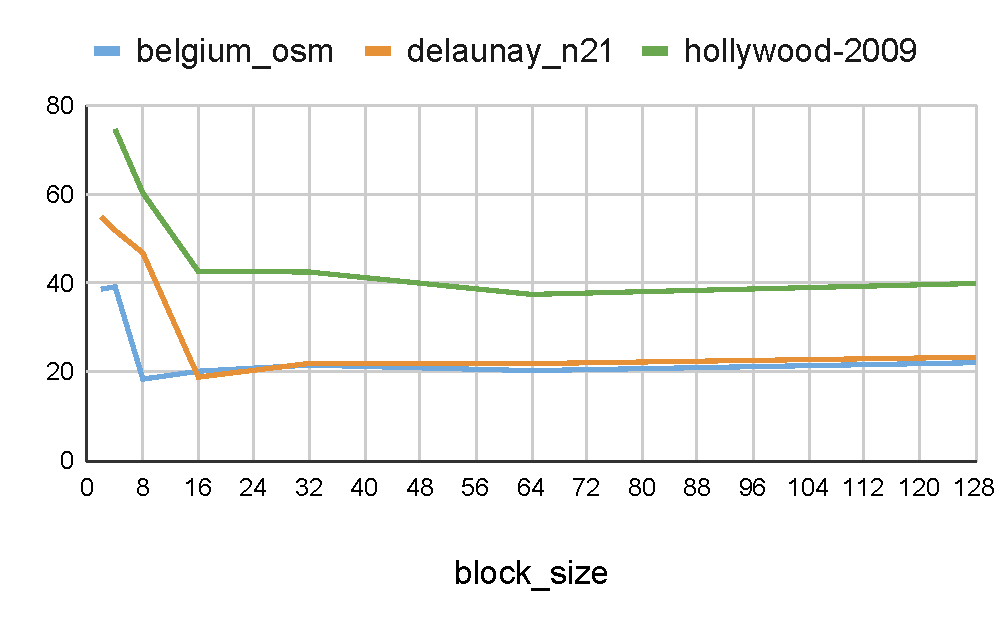
\includegraphics[width=0.7\textwidth]{Chapters/Figures/plots/block_size_edge_insertion.pdf}
    \caption{Block size benchmark: Total edge insertion time in milliseconds.}
    \label{fig:block_size_edge_insertion}
\end{figure}

% Regarding edge insertion times, we see a decrease in insertion times (Figure~\ref{fig:block_size_edge_insertion}) when increasing the block-size up to 16. This makes sense given that small block-sizes require allocating new blocks often while inserting edges. However, for block sizes exceeding 16, insertion times remain relatively constant. This is particularly apparent in the belgium\_osm and delaunay\_n21 datasets, where adjacency lists (including the newly inserted edges) are expected to fit entirely within a block-size of 16. Concerning the hollywood-2009 graph (which contains large adjacency lists), the diminishing returns in insertion times with increasing block-size might be attributed to the constraints imposed by the size of the \gls{GPU} cache-lines. Despite the potential to fit more adjacencies within a single block, the amount of data fetchable at once is bounded by the cache-line size, typically around 128 bytes. Note that using weighted edges, each edge inside a block takes up 8 bytes, meaning that a block-size of 16, leads to blocks of 128 bytes.

Regarding edge insertion times, we see a decrease in insertion times (Figure~\ref{fig:block_size_edge_insertion}) when increasing the block size up to 16. This makes sense given that small block sizes result in frequent block allocations while inserting edges. For block sizes exceeding 16, insertion times remain relatively constant. This is expected since the newly inserted edges are expected to fit entirely within the last block of the corresponding adjacency list. The same applies to the denser hollywood-2009 graph. Although graph construction times benefit from larger block sizes, the key consideration for edge insertion efficiency is ensuring that there is enough space within the last block to accommodate new edges, thereby avoiding the need for frequent block allocations.

\begin{figure}
    \centering
    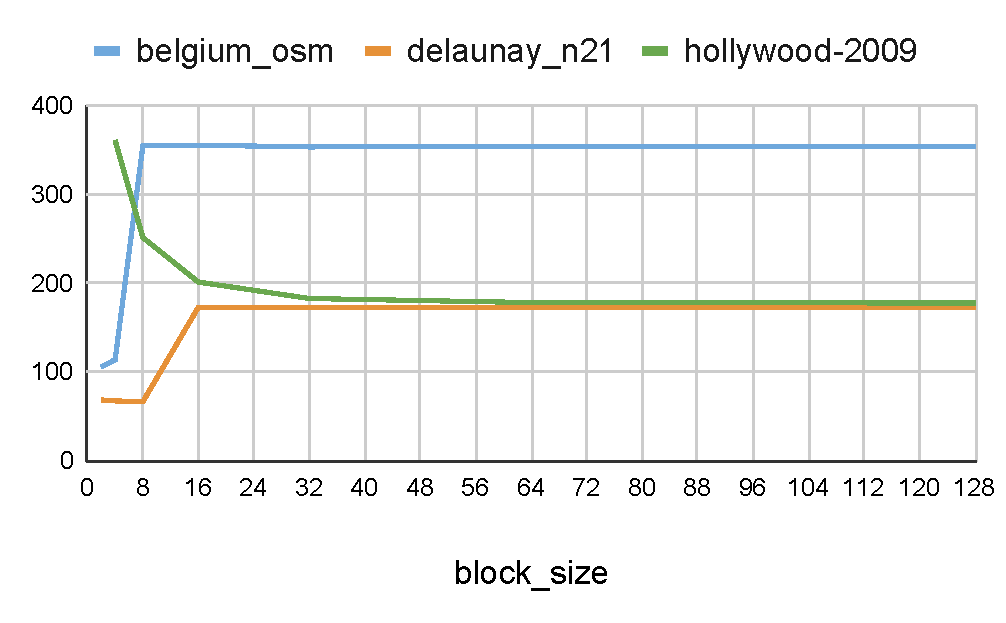
\includegraphics[width=0.7\textwidth]{Chapters/Figures/plots/block_size_sssp.pdf}
    \caption{Block size benchmark: Mean SSSP execution time in milliseconds.}
    \label{fig:block_size_edge_sssp}
\end{figure}

% Many reads / queries to data-structure
% Exact correct block size -> good locality
% consecutive threads search for consecutive neighbours of given source vertex during advance
% Small block size doen't matter, because blocks are next to each other
% Larger block size -> requires more memory fetches (remember cach line of 128 bytes, and blocks of 16 bytes)
% Performance doesnt get worse because the same number of memory fetches are used
As we can see in Figure~\ref{fig:block_size_edge_sssp}, the average \gls{SSSP} execution times see a significant increase when we increase the block size from 4 to 8 and from 8 to 16 while processing the belgium\_osm and delaunay\_n21 graphs respectively. One possible explanation is related to the manner in which \gls{GPU}s fetch global data in blocks of 128 bytes. The \gls{SSSP} makes extensive use of the advance operator. This operator performs a lot of consecutive reads to the graph's data structure. Consecutive threads search for consecutive neighbors of a given source vertex. This means that if an ideal block size is used (2/4 for belgium\_osm and 8 for delaunay\_n21, given their respective average degrees of 1 and 5), we can take maximum advantage of the 128-byte cache lines. The same is also true for even smaller block sizes. Given that, typically, blocks comprising a vertex's adjacency list are stored consecutively, they also benefit from coalesced memory reads. If we double the block size from the ideal value, this leads to a lot of unused positions in each block. In turn, each global memory access fetches half as much useful data. This can result in half (or less) as many cache hits, leading to significantly worse performance. The hollywood-2009 graph on the other hand, benefits from using large block sizes. Given its large average degree of 105, using larger blocks leads to less time spent iterating over multiple blocks.

We can conclude that there is not an ideal block size, as it depends on the characteristics of the graph we are processing. The ideal block size seems to be tied to the average and maximum degrees of a given graph. Regardless, for the types of graphs we'll be using in this evaluation, we can see that a block size of 8 or 16, seems to yield good general performance. For this reason, we will adopt a default block size of 8, which we may adjust as needed based on specific graph characteristics and performance considerations.










\paragraph{\textbf{Graph Initialization}.} From Table~\ref{tab:m1_graph_init} (containing the results from Machine 1), we can see that Marrow-Graph has overall faster graph initialization times than Gunrock and just slightly slower times than Ligra. Hornet shows relatively faster initialization times than Marrow-Graph, Gunrock, and Ligra. FaimGraph has some of the best initialization times for graphs like belgium\_osm and roadNet-CA, but shows similar initialization times to Marrow-Graph for the dense graph hollywood-2009, and fails to load road\_usa. Overall, Marrow-Graph offers quite satisfactory graph initialization times. The results obtained using Machine 2 (Table~\ref{tab:m2_graph_init}) are very similar, with the exception of Ligra, which performs significantly better due to a faster processor.

\definecolor{lightred}{RGB}{220, 180, 180}


\begin{table}%[htbp]
  \centering
  \small
    \begin{tabular}{|l|ccccc|}
    \hline
          & \text{delaunay\_n21} & \text{roadNet-CA} & \text{hollywood-2009} & \text{belgium\_osm} & \text{road\_usa} \\
    \hline
    \hline
    marrow-graph & 1643+118 & 853+112 & 14260+378 & 553+97 & 11031+778 \\
    gunrock & \cellcolor{lightred}2191 & \cellcolor{lightred}1038 & \cellcolor{lightred}19515 & 512 & 10082 \\
    hornet & 1300 & 671 & 10321 & 455 & 6557 \\
    ligra & 1730 & 855 & 13300 & 518 & 11100 \\
    faimgraph & 1464 & 130 & 14600 & 71 & \text{-} \\
    \hline
    \end{tabular}%
    \caption{Machine 1: Graph initialization times in milliseconds (red: slower than marrow-graph, marrow-graph: construction time + upload).}

  \label{tab:m1_graph_init}%
\end{table}%



% \begin{table}%[htbp]
%   \centering
%   \small
%     \begin{tabular}{|l|ccccc|}
%     \hline
%            & \text{delaunay\_n21} & \text{roadNet-CA} & \text{hollywood-2009} & \text{belgium\_osm} & \text{road\_usa} \\
%     \hline
%     \hline
%     marrow-graph & 1482 & 837 & 12326 & 583 & 9630 \\
%     gunrock & \cellcolor{lightred}1717 & 741 & \cellcolor{lightred}15358 & 419 & 8141 \\
%     hornet & 969 & 535 & 7314 & 364 & 4943 \\
%     ligra & 384 & 193 & 2960 & 117 & 2360 \\
%     faimgraph & 362 & 167 & 2896 & 87 & \text{-} \\
%     \hline
%     \end{tabular}%
%     \caption{Machine 2: Graph initialization times in milliseconds (red: slower than marrow-graph).}

%   \label{tab:m2_graph_init}%
% \end{table}%


\begin{table}%[htbp]
  \centering
  \small
    \begin{tabular}{|l|ccccc|}
    \hline
           & \text{delaunay\_n21} & \text{roadNet-CA} & \text{hollywood-2009} & \text{belgium\_osm} & \text{road\_usa} \\
    \hline
    \hline
    marrow-graph & 1356+100 & 733+89 & 11468+161 & 491+82 & 9146+261 \\
    gunrock & \cellcolor{lightred}1717 & 741 & \cellcolor{lightred}15358 & 419 & 8141 \\
    hornet & 969 & 535 & 7314 & 364 & 4943 \\
    ligra & 384 & 193 & 2960 & 117 & 2360 \\
    faimgraph & 362 & 167 & 2896 & 87 & \text{-} \\
    \hline
    \end{tabular}%
    \caption{Machine 2: Graph initialization times in milliseconds (red: slower than marrow-graph, marrow-graph: construction time + upload).}

  \label{tab:m2_graph_init}%
\end{table}%

\paragraph{\textbf{Graph Updates}.} Figures~\ref{fig:lmarrow-graph_insertion_heat_plot},~\ref{fig:hornet_insertion_heat_plot}, and~\ref{fig:faimgraph_insertion_heat_plot} show the edge insertion rates obtained by each framework on Machine 2 (we achieved similar results on Machine 1). Each heat plot contains the insertion rates for inserting $N$ edges, where $N = \{10^k : k \in \{0,1,2,...,6\}\}$, using batches of size $B$, where $B = \{10^k : k \in \{0,1,2,\ldots,6\} \land 10^k \leq N\}$
. This means that we measure both the insertion rates for inserting single large batches, as well as multiple smaller batches. 

As we can see in Figure~\ref{fig:lmarrow-graph_insertion_heat_plot}, Marrow-Graph has a fairly consistent edge insertion rate, for any size of batch and any number of inserted edges, around $4.0 * 10^5$ \textit{edges/second}. For larger batches such as $10^6$, it achieves rates up to $8.85 * 10^6$ \textit{edges/second}. 

Hornet (Figure~\ref{fig:hornet_insertion_heat_plot}), displays significantly lower insertion rates for batch sizes up to $10^2$. Using a batch size of $10^3$, we see similar insertion rates for a number of inserted edges up to $10^4$, and better insertion rates by Hornet for larger numbers of inserted edges. For batch sizes over $10^3$, Hornet offers better insertion rates than Marrow-Graph. This makes sense given that Marrow-Graph performs the updates on the host and synchronizes the changes to the device, while Hornet performs the updates directly on the device. This means that smaller batch sizes can be more efficiently updated on the host and later synchronized to the device, while larger batches can be inserted in parallel directly on the device more efficiently.

FaimGraph (Figure~\ref{fig:faimgraph_insertion_heat_plot}), offers the best insertion rates for medium to large batch sizes. For small batch sizes of $1$ and $10$, Marrow-Graph achieves comparable, and in some instances, better insertion rates than FaimGraph. For batch sizes of $10^2$ and bigger, FaimGraph outperforms both Marrow-Graph and Hornet. This is most likely related to FaimGraph's optimized memory manager.

\begin{figure}
    \begin{subfigure}{0.5\textwidth}
        \centering
        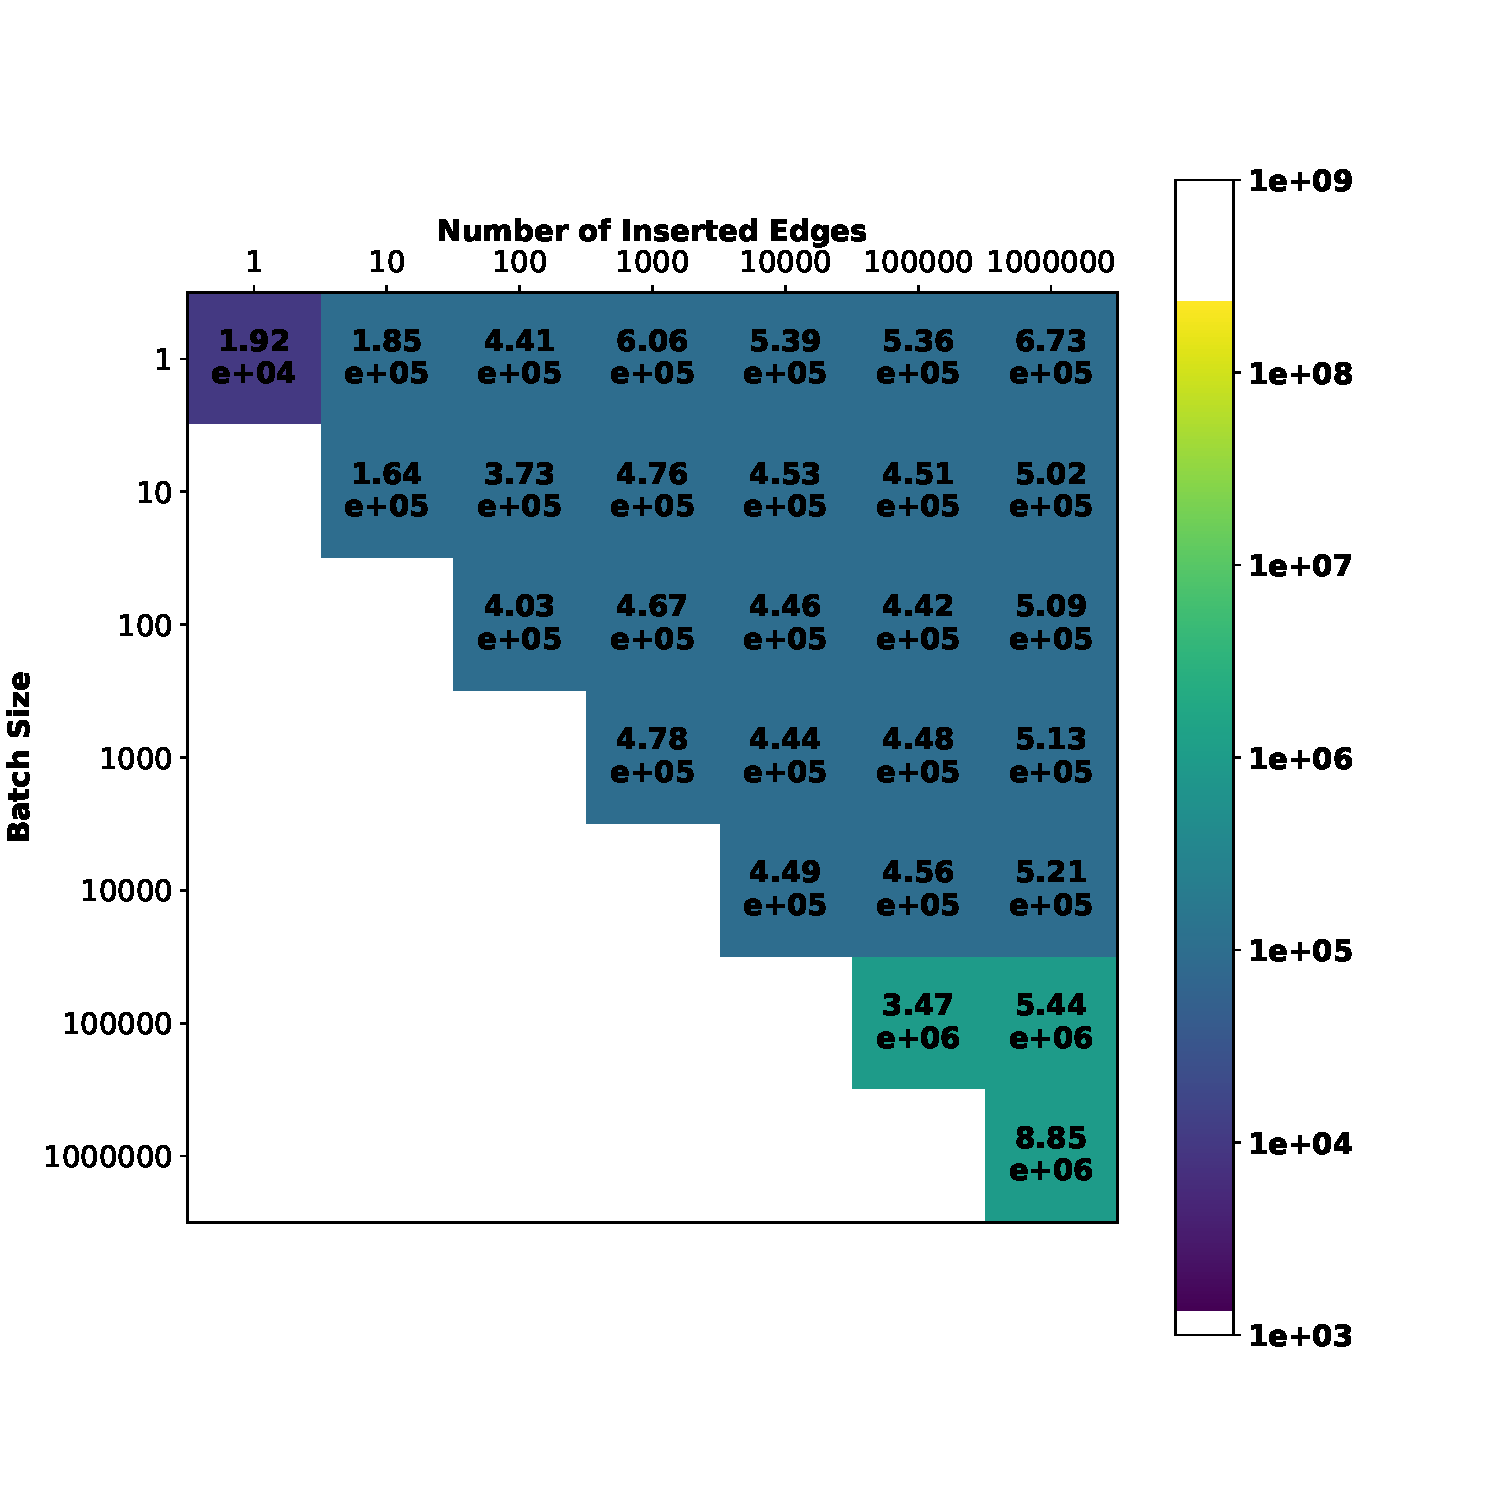
\includegraphics[width=\linewidth]{Chapters/Figures/plots/lmarrow-graph_edge_update_belgium_osm_benchmark.pdf}
        \caption{belgium\_osm}
    \end{subfigure}%
    \begin{subfigure}{0.5\textwidth}
        \centering
        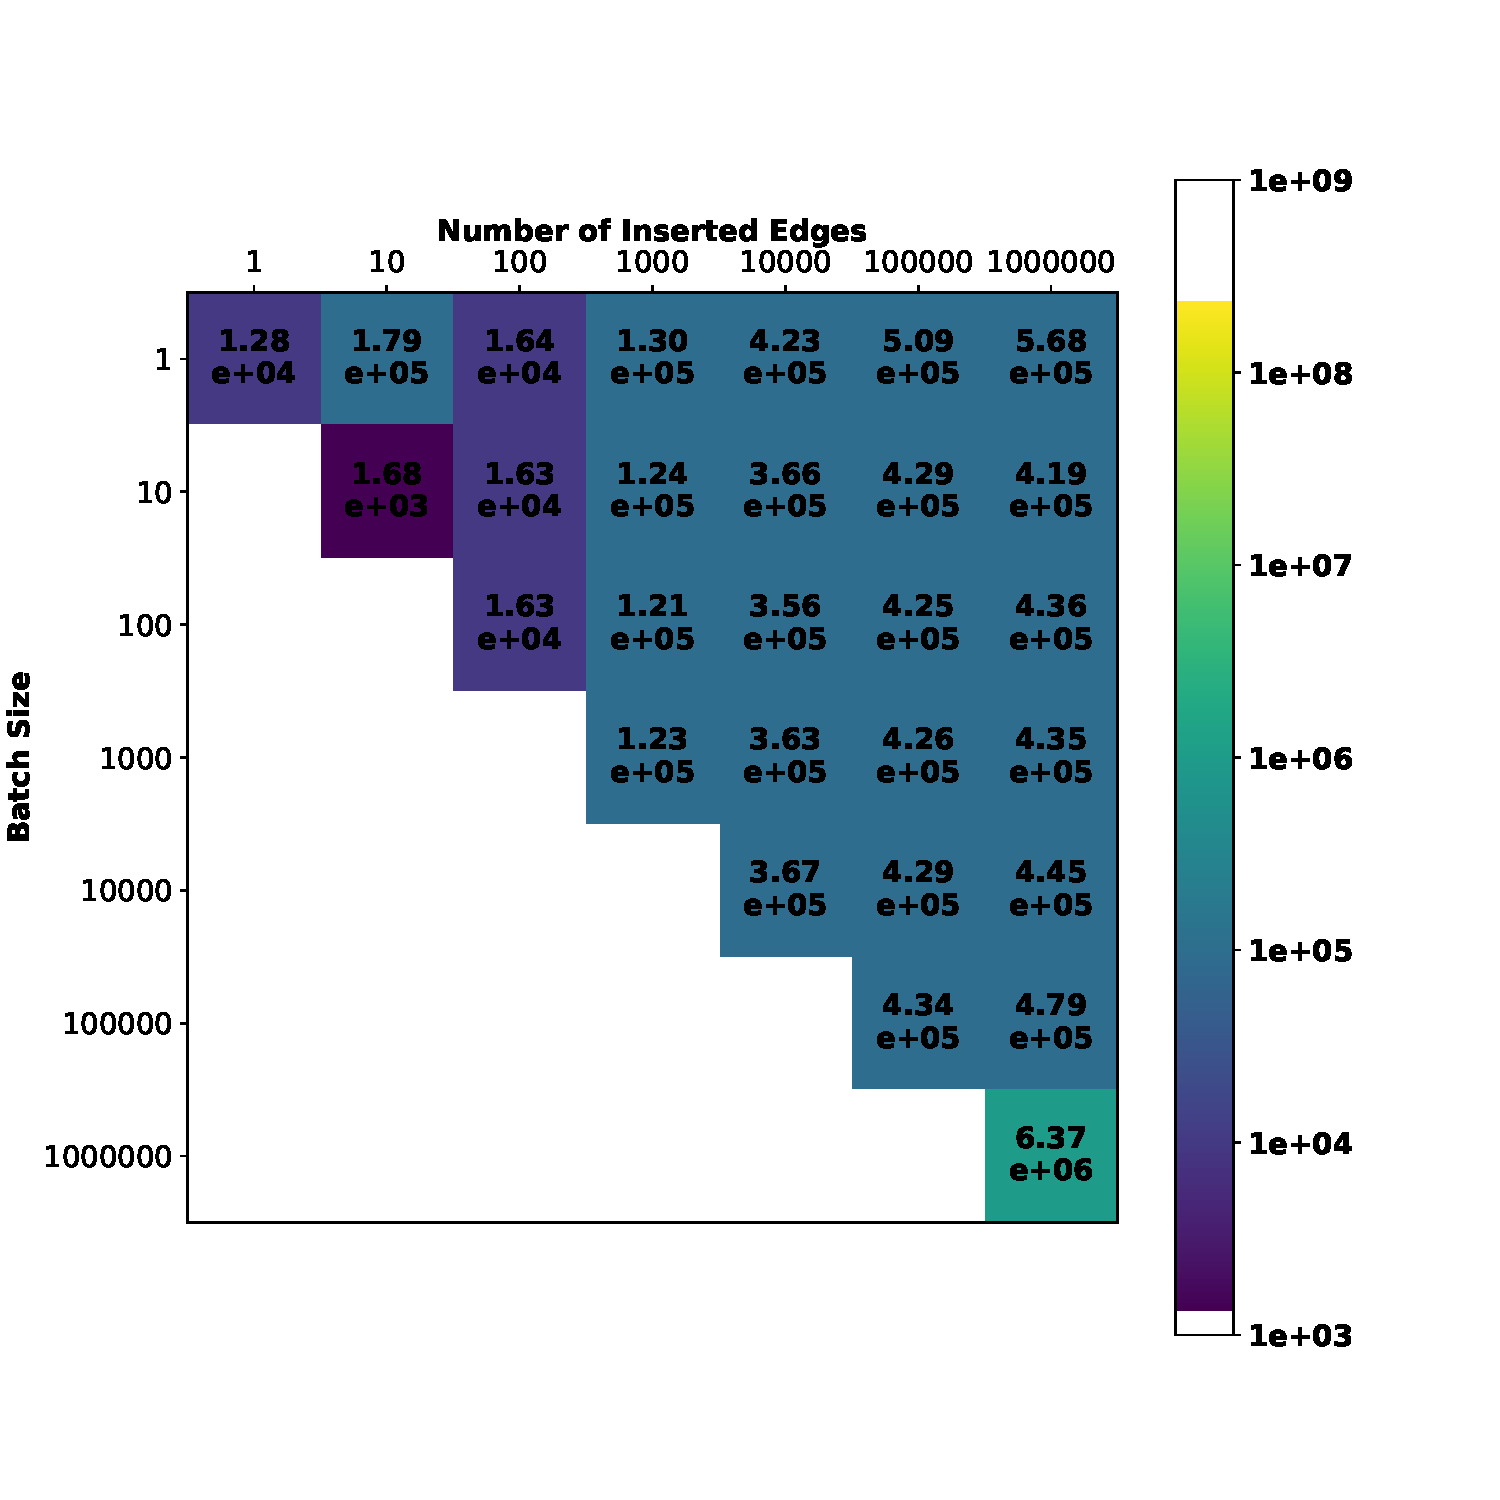
\includegraphics[width=\linewidth]{Chapters/Figures/plots/lmarrow-graph_edge_update_delaunay_n21_benchmark.pdf}
        \caption{delaunay\_m21}
    \end{subfigure}%
    \caption{Machine 2: Marrow-Graph edge insertion rates (edge/second).}
    \label{fig:lmarrow-graph_insertion_heat_plot}
\end{figure}

\begin{figure}
    \begin{subfigure}{0.5\textwidth}
        \centering
        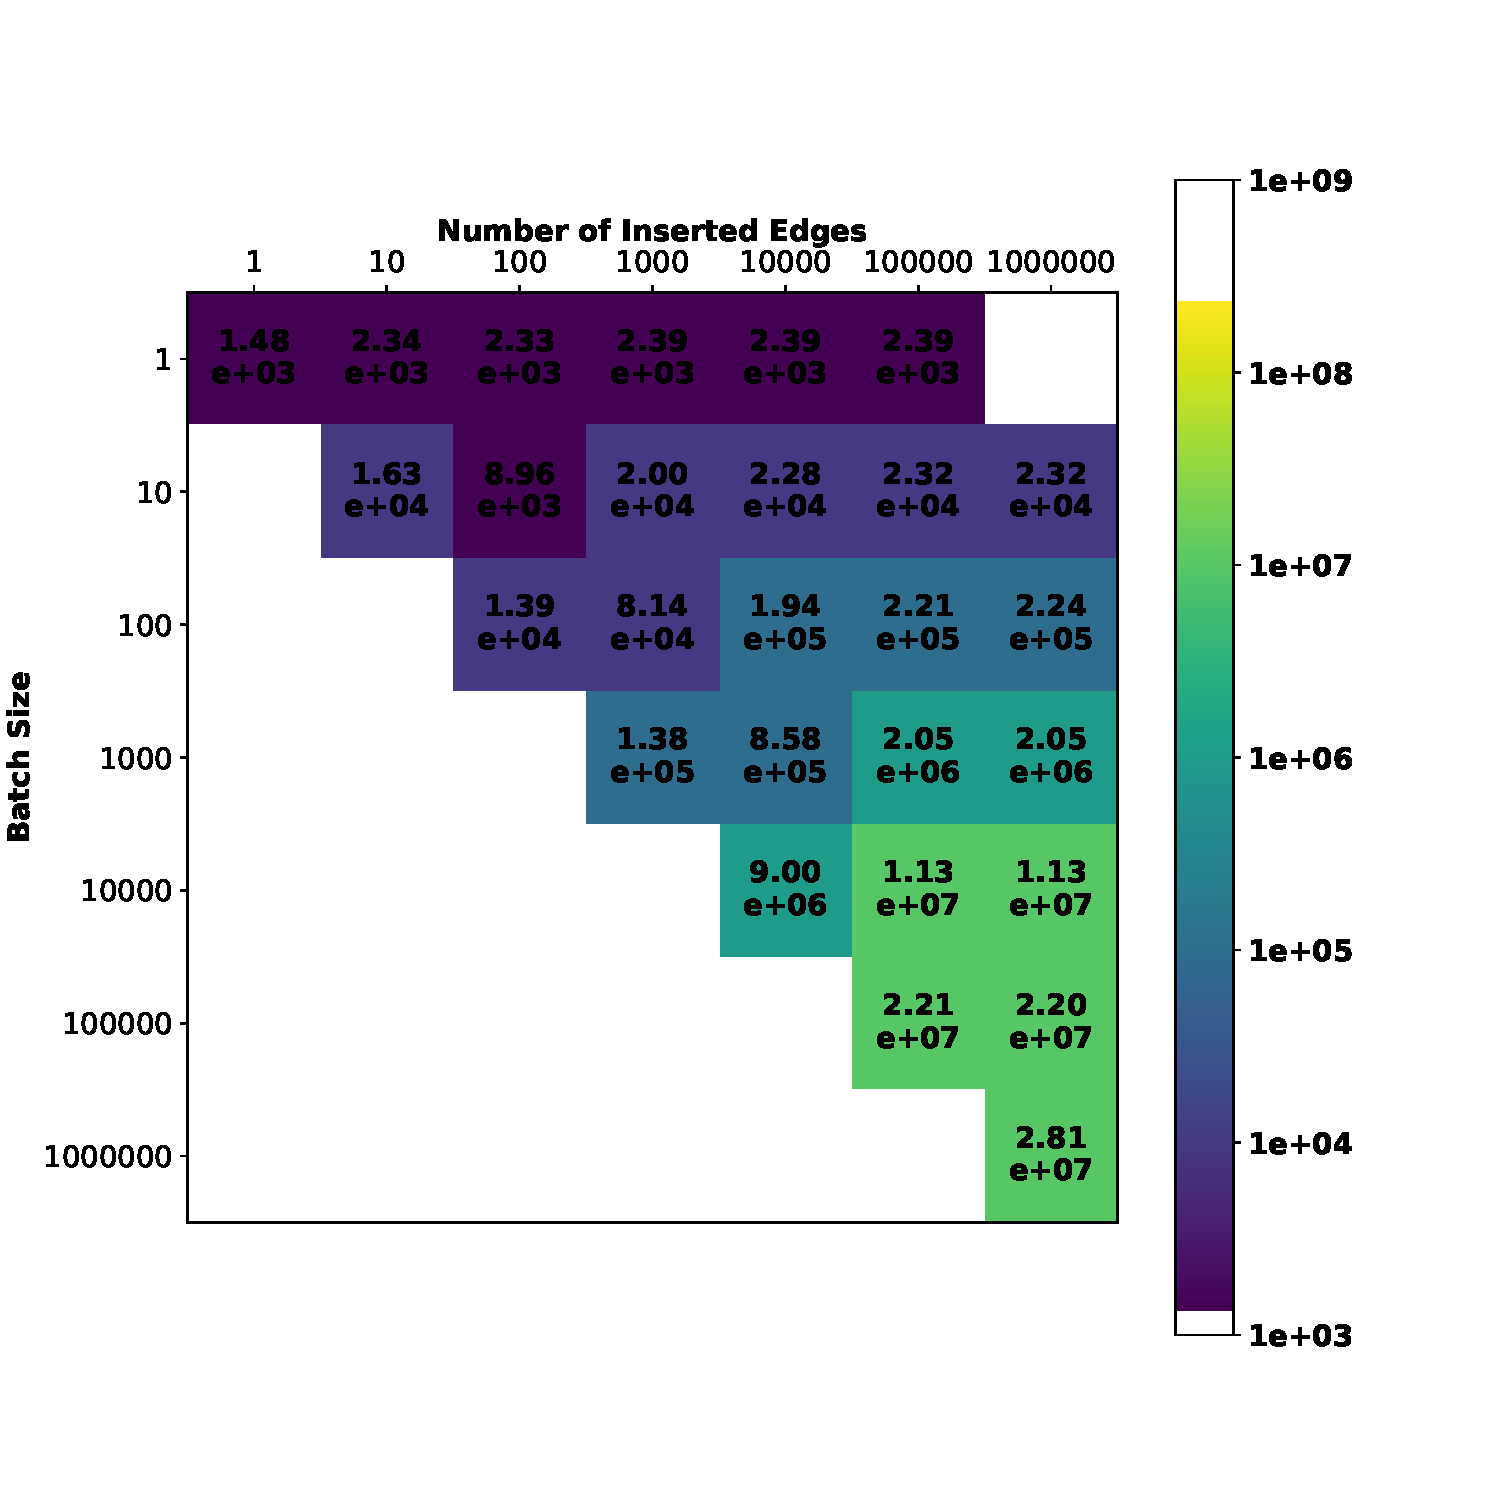
\includegraphics[width=\linewidth]{Chapters/Figures/plots/hornet_edge_update_belgium_osm_benchmark.pdf}
        \caption{belgium\_osm}
    \end{subfigure}%
    \begin{subfigure}{0.5\textwidth}
        \centering
        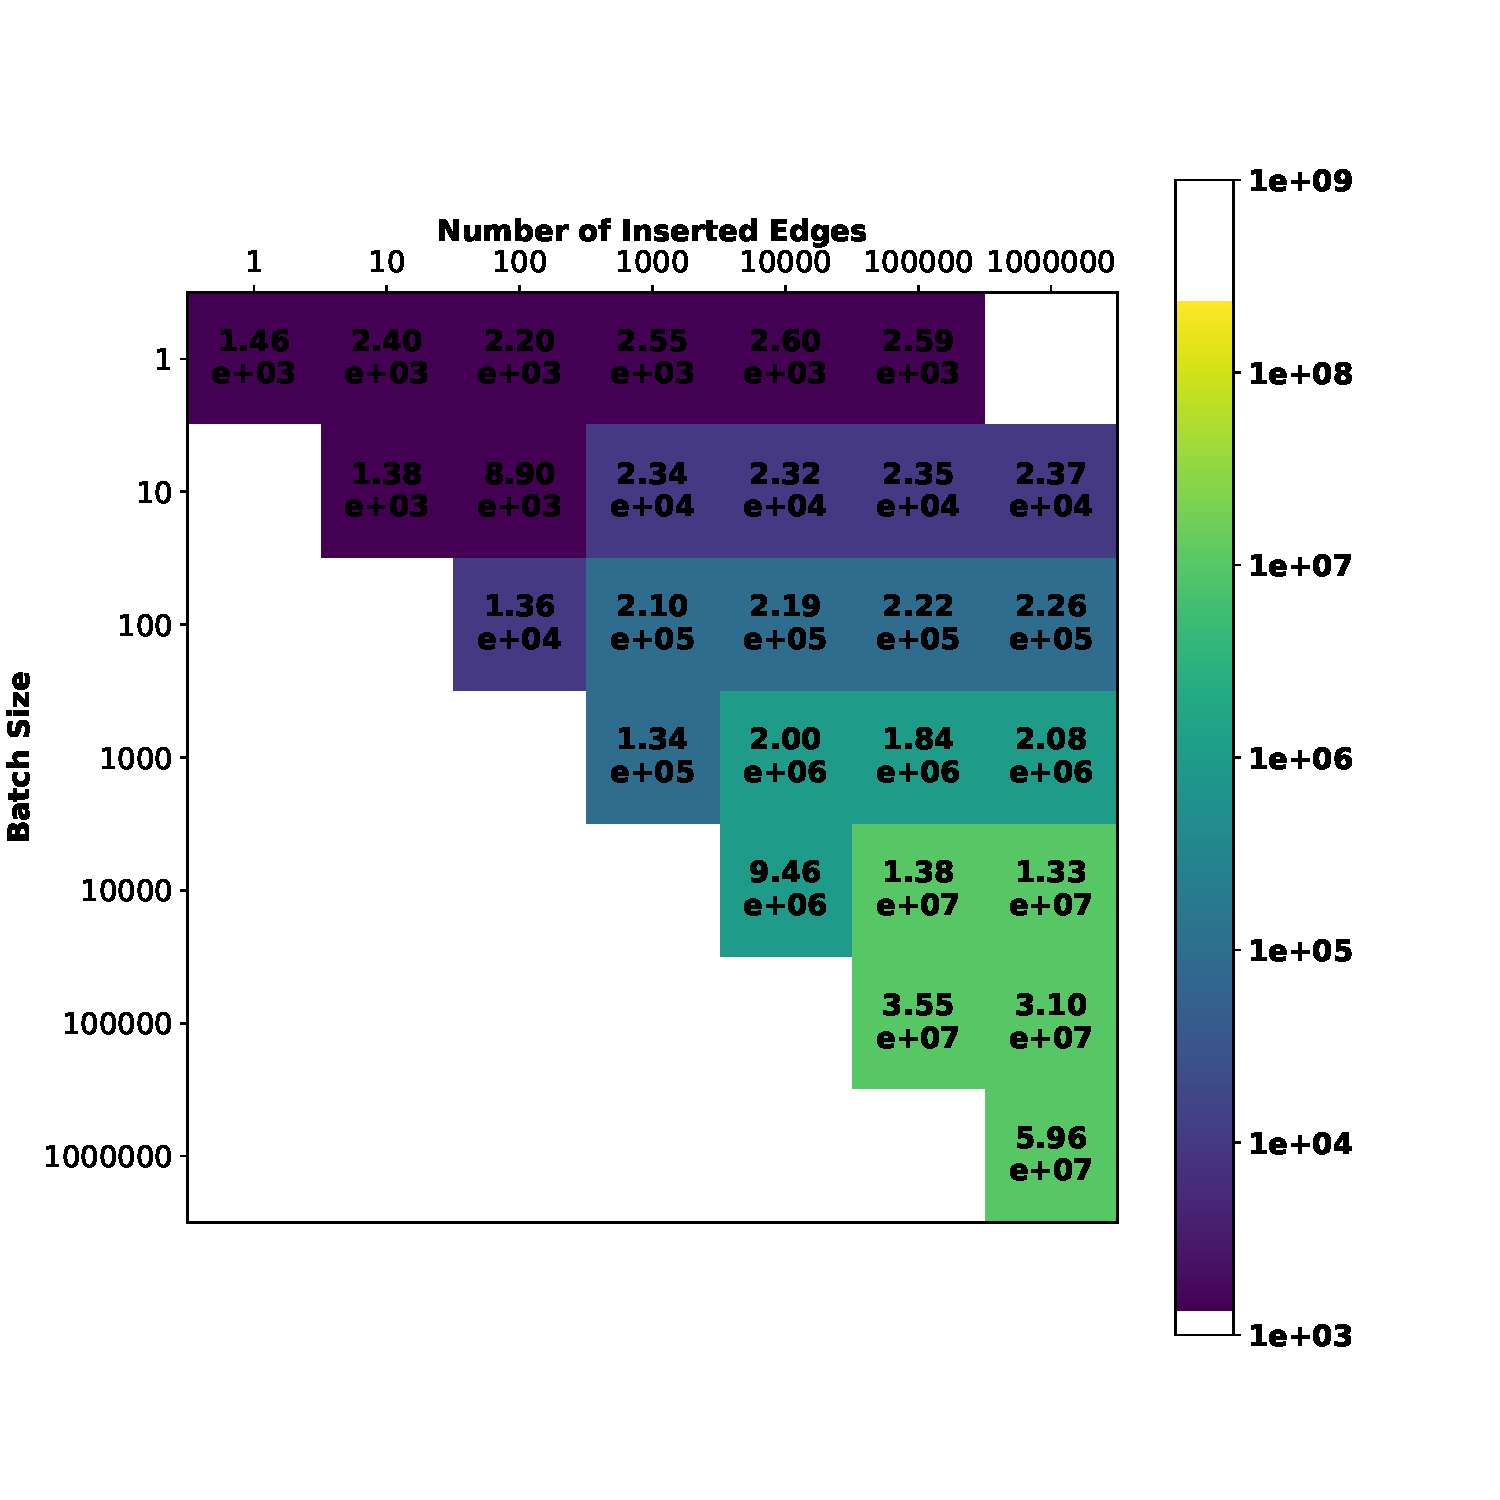
\includegraphics[width=\linewidth]{Chapters/Figures/plots/hornet_edge_update_delaunay_n21_benchmark.pdf}
        \caption{delaunay\_m21}
    \end{subfigure}%
    \caption{Machine 2: Hornet edge insertion rates (edge/second).}
    \label{fig:hornet_insertion_heat_plot}
\end{figure}

\begin{figure}
    \begin{subfigure}{0.5\textwidth}
        \centering
        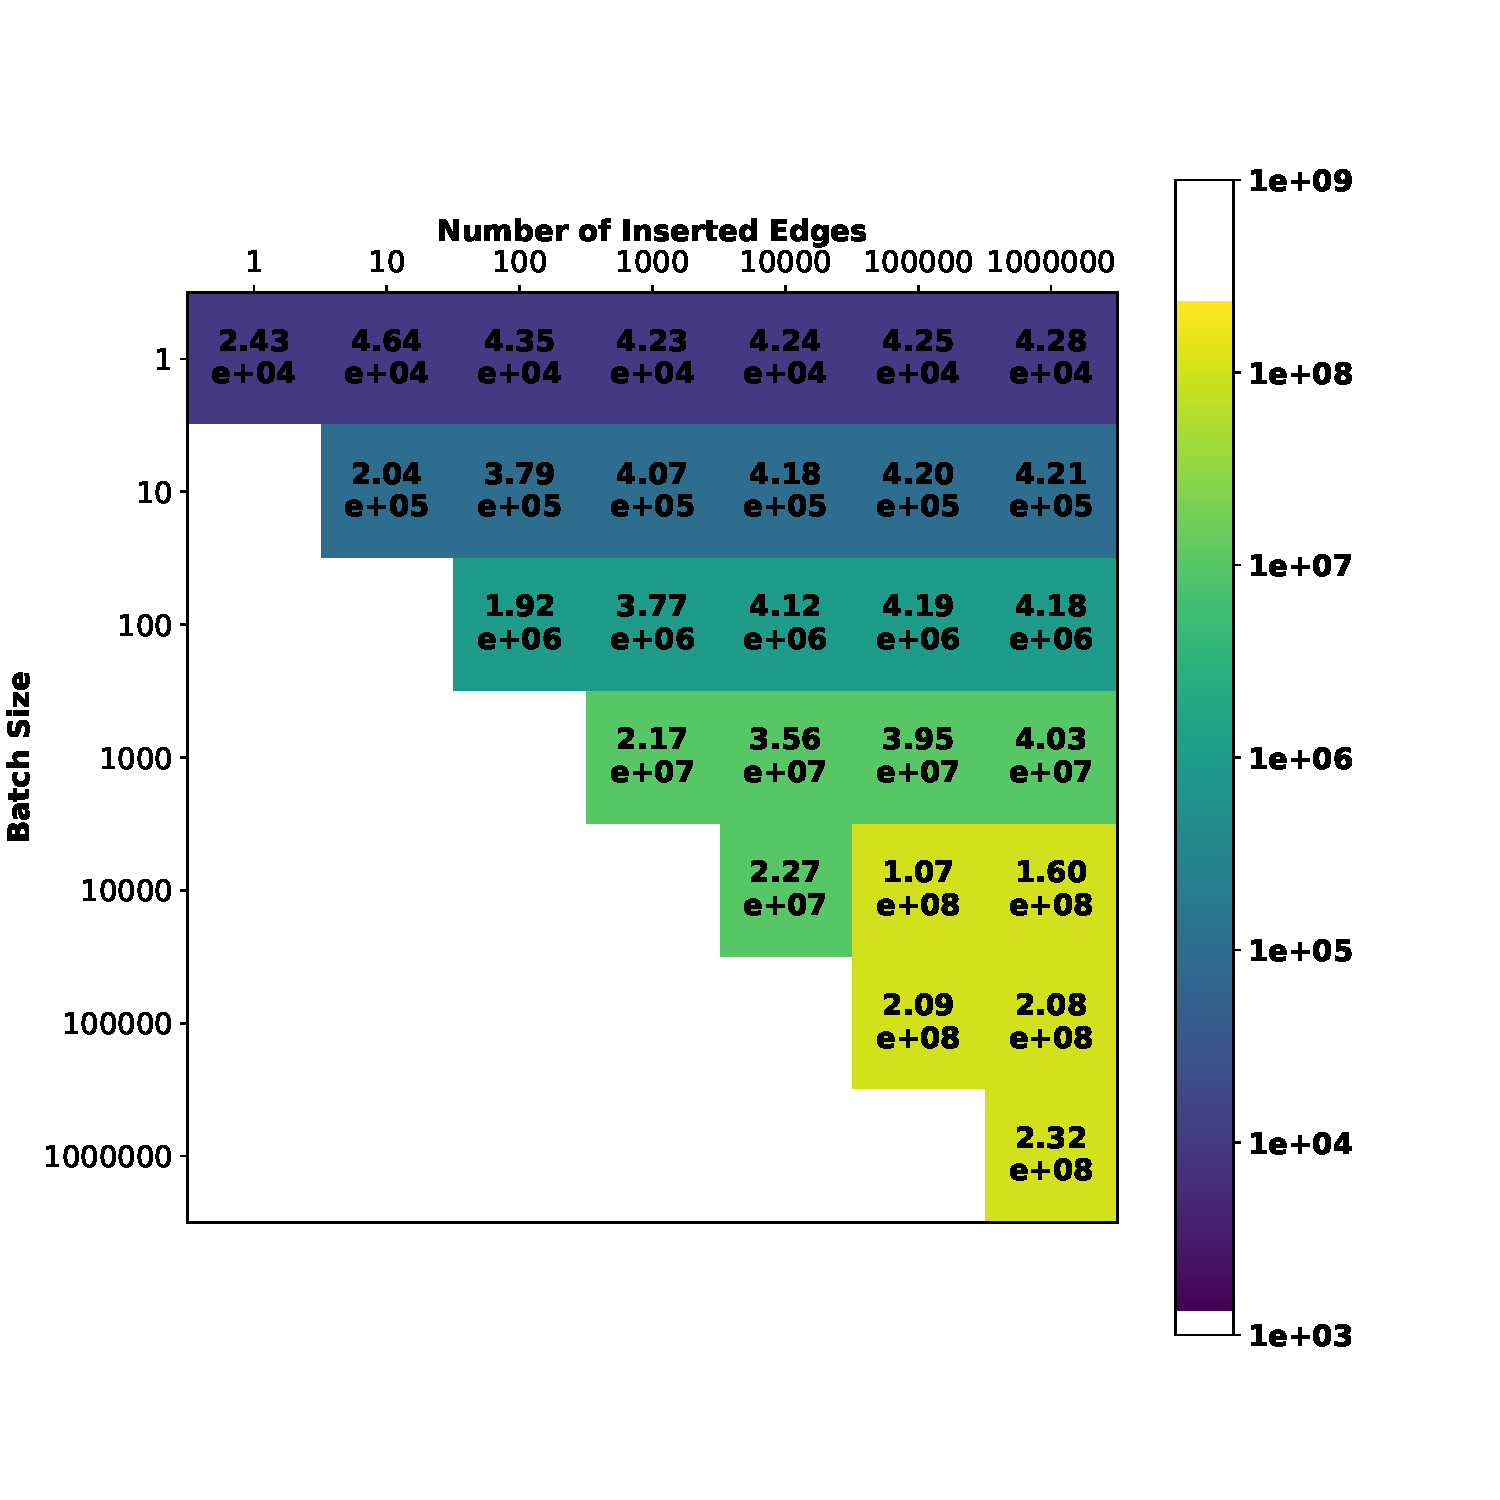
\includegraphics[width=\linewidth]{Chapters/Figures/plots/faimgraph_edge_update_belgium_osm_benchmark.pdf}
        \caption{belgium\_osm}
    \end{subfigure}%
    \begin{subfigure}{0.5\textwidth}
        \centering
        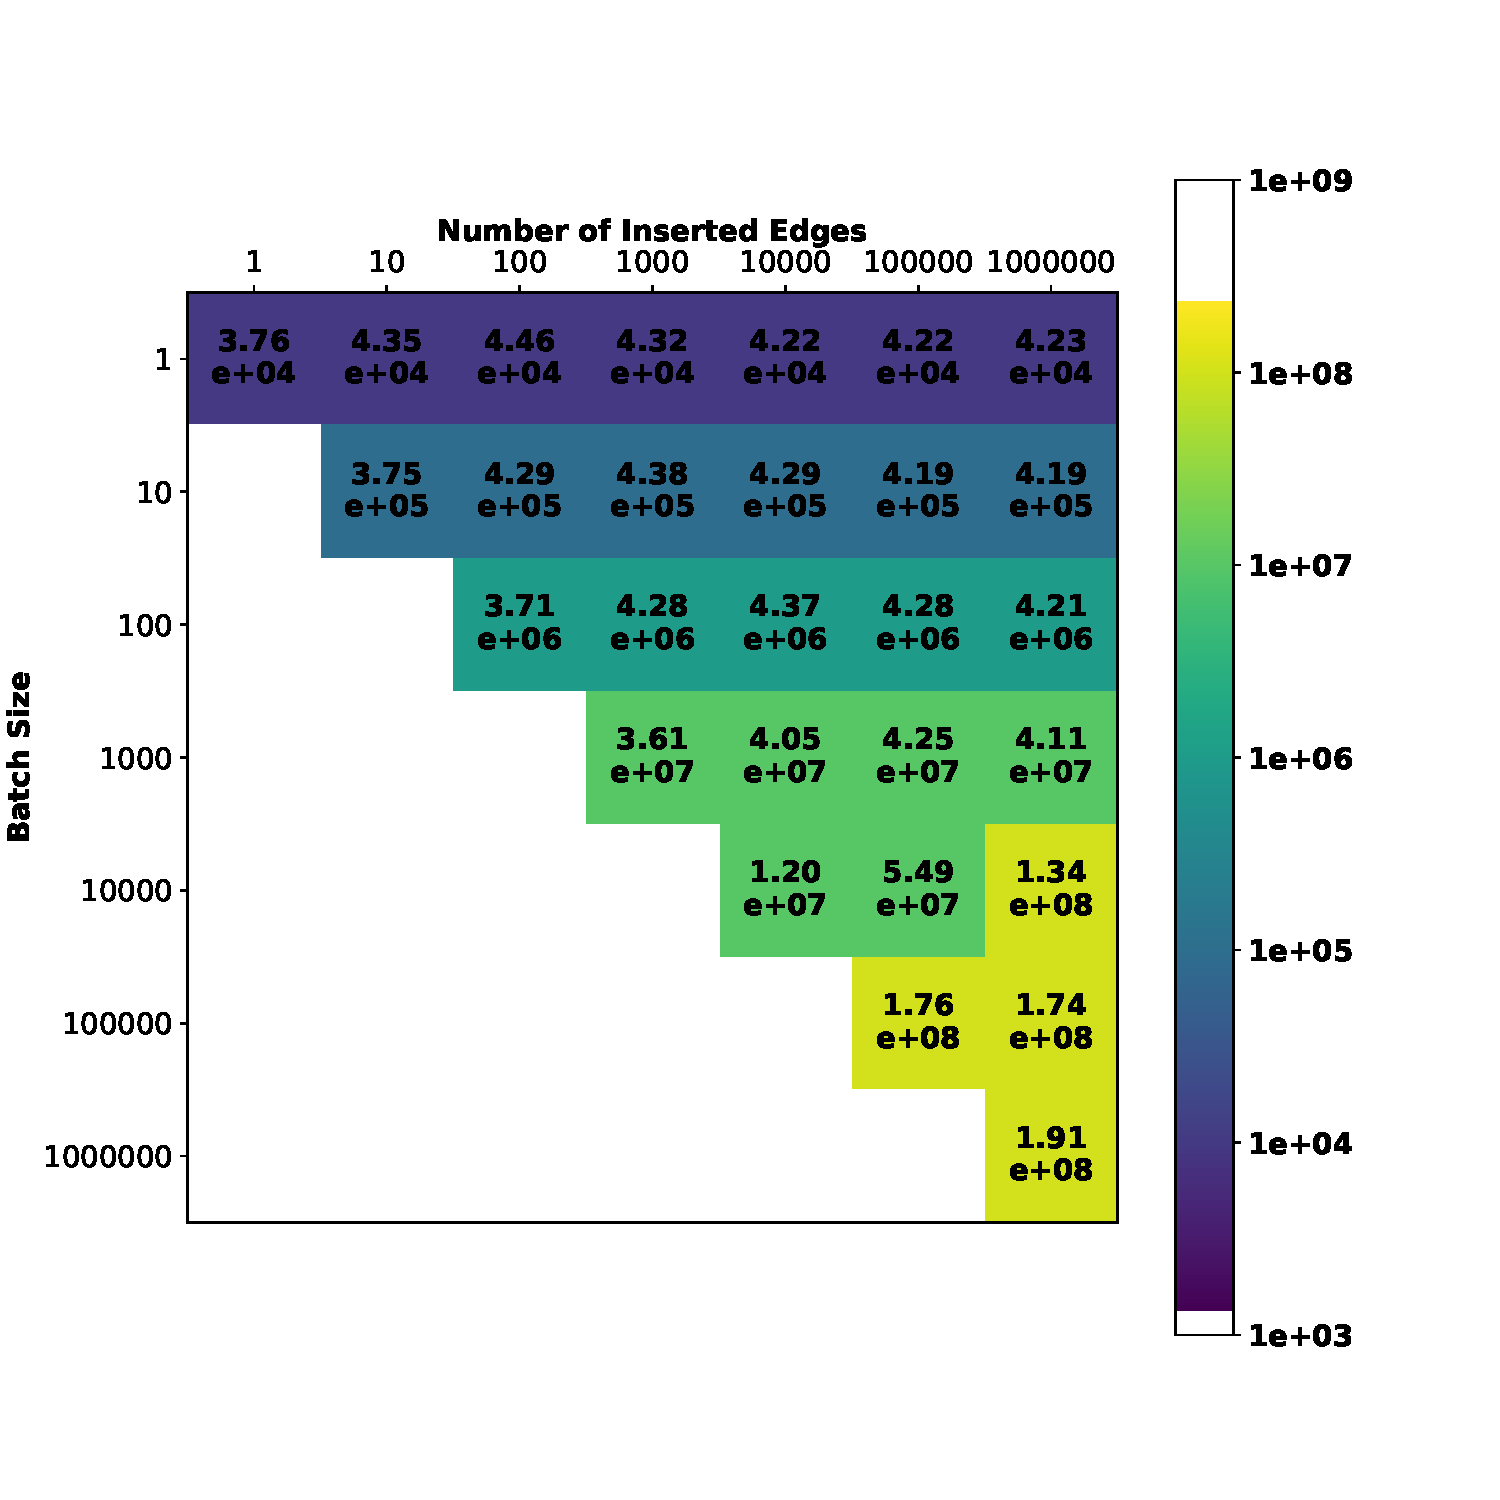
\includegraphics[width=\linewidth]{Chapters/Figures/plots/faimgraph_edge_update_delaunay_n21_benchmark.pdf}
        \caption{delaunay\_m21}
    \end{subfigure}%
    \caption{Machine 2: FaimGraph edge insertion rates (edge/second).}
    \label{fig:faimgraph_insertion_heat_plot}
\end{figure}



\definecolor{lightred}{RGB}{220, 180, 180}
\definecolor{lightgreen}{RGB}{180, 220, 180}
\definecolor{lightergreen}{RGB}{220, 255, 220}
\definecolor{lightyellow}{RGB}{220, 220, 180}

\begin{table}%[htbp]
  \centering
  \footnotesize
    \begin{tabular}{|l|SSSSS|}
    
    \hline
          & \text{delaunay\_n21} & \text{roadNet-CA} & \text{hollywood-2009} & \text{belgium\_osm} & \text{road\_usa} \\
    
    \hline
    \hline

    & \multicolumn{5}{c|}{SpMV} \\
    \hline
    marrow-graph & 3.85 & 1.63 & 46.79 & 1.03 & 30.18 \\
    faimgraph & \text{-} & \cellcolor{lightred}1.82 & \text{-} & \cellcolor{lightred}1.31 & \text{-} \\
    hornet & 2.66 & \cellcolor{lightred}1.99 & 40.21 & 1.01 & 16.36 \\
    gunrock & 2.52 & 1.51 & 25.96 & \cellcolor{lightred}1.07 & 12.79 \\

    \hline
    
    & \multicolumn{5}{c|}{BFS} \\
    \hline
    marrow-graph & 160.87 & 152.43 & 240.69 & 338.05 & 5283.12 \\
    faimgraph & 84.60 & 70.73 & 88.89 & 134.12 & \text{-} \\
    hornet & 39.27 & 38.78 & 21.10 & 95.66 & 470.18 \\
    gunrock & 79.50 & 73.12 & 112.51 & 167.90 & 802.97 \\
    ligra & 41.40 & 34.70 & 49.80 & 30.20 & 519.00 \\
    
    \hline

    & \multicolumn{5}{c|}{SSSP} \\
    \hline
    marrow-graph & 167.13 & 156.49 & 252.31 & 337.76 & 5398.88 \\
    hornet & 46.25 & 40.93 & 27.59 & 96.26 & 496.75 \\
    gunrock & 85.52 & 78.49 & 108.98 & 188.52 & 880.10 \\
    ligra & 70.20 & 65.40 & 201.00 & 40.80 & 689.00 \\

    \hline

    & \multicolumn{5}{c|}{PR} \\
    \hline
    marrow-graph & 18.49 & 27.82 & 815.60 & 14.84 & 123.09 \\
    hornet & 6.75 & 20.70 & 130.31 & 9.88 & 50.34 \\
    gunrock & 9.04 & 13.61 & 266.05 & 6.02 & 46.45 \\
    ligra & \cellcolor{lightred}1280.00 & \cellcolor{lightred}1710.00 & \cellcolor{lightred}15700.00 & \cellcolor{lightred}1640.00 & \cellcolor{lightred}32100.00 \\

    \hline

    & \multicolumn{5}{c|}{TC} \\
    \hline
    marrow-graph & 58.78 & 7.85 & 12915.90 & 4.24 & 136.00 \\
    faimgraph & 7.03 & 2.05 & \text{-} & 1.24 & \text{-} \\
    gunrock & 10.58 & 2.79 & \text{-} & 1.66 & 28.92 \\
    ligra & \cellcolor{lightred}128.00 & \cellcolor{lightred}59.40 & \cellcolor{lightred}52600.00 & \cellcolor{lightred}46.10 & \cellcolor{lightred}782.00 \\

    \hline
    
    \end{tabular}%
  \caption{Machine 1: Algorithmic execution times in milliseconds (red: slower than marrow-graph).}

  \label{tab:m1_algo}%
\end{table}%




\definecolor{lightred}{RGB}{220, 180, 180}
\definecolor{lightgreen}{RGB}{180, 220, 180}
\definecolor{lightergreen}{RGB}{220, 255, 220}
\definecolor{lightyellow}{RGB}{220, 220, 180}
            
\begin{table}%[htbp]
  \centering
  \footnotesize
    \begin{tabular}{|l|SSSSS|}
    
    \hline
          & \text{delaunay\_n21} & \text{roadNet-CA} & \text{hollywood-2009} & \text{belgium\_osm} & \text{road\_usa} \\
    
    \hline
    \hline

    & \multicolumn{5}{c|}{SpMV} \\
    \hline
    marrow-graph & 1.203 & 0.433 & 18.918 & 0.395 & 8.658 \\
    faimgraph & \text{-} & \text{-} & \text{-} & \text{-} & \text{-} \\
    hornet & 1.173 & \cellcolor{lightred}4.06 & \cellcolor{lightred}26.139 & \cellcolor{lightred}3.939 & \cellcolor{lightred}14.211 \\
    gunrock & 1.106 & \cellcolor{lightred}0.754 & 11.626 & \cellcolor{lightred}0.647 & 5.430 \\

    \hline
    
    & \multicolumn{5}{c|}{BFS} \\
    \hline
    marrow-graph & 104.478 & 100.664 & 130.023 & 233.658 & 2763.38 \\
    faimgraph & 44.480 & 38.394 & 22.711 & 84.602 & \text{-} \\
    hornet & 65.503 & 78.217 & 9.665 & 177.849 & 997.135 \\
    gunrock & 25.939 & 23.754 & 27.636 & 52.818 & 257.659 \\
    ligra & 28.0 & 25.6 & 17.2 & 29.9 & 303.0 \\

    
    \hline

    & \multicolumn{5}{c|}{SSSP} \\
    \hline
    marrow-graph & 107.062 & 101.855 & 135.285 & 236.958 & 2795.07 \\
    hornet & 77.0035 & 88.643 & 15.863 & 193.334 & 1093.71 \\
    gunrock & 30.127 & 27.333 & 35.425 & 62.584 & 299.02 \\
    ligra & 33.4 & 31.2 & \text{-} & 35.8 & 361.0 \\


    \hline

    & \multicolumn{5}{c|}{PR} \\
    \hline
    marrow-graph & 5.277 & 9.261 & 319.25 & 5.286 & 33.614 \\
    hornet & \cellcolor{lightred}8.263 & \cellcolor{lightred}14.878 & 51.627 & \cellcolor{lightred}8.868 & 28.014 \\
    gunrock & 2.858 & 4.884 & 78.519 & 2.554 & 15.535 \\
    ligra & \cellcolor{lightred}454.0 & \cellcolor{lightred}477.0 & \cellcolor{lightred}5180.0 & \cellcolor{lightred}410.0 & \cellcolor{lightred}12000.0 \\


    \hline

    & \multicolumn{5}{c|}{TC} \\
    \hline
    marrow-graph & 18.191 & 1.866 & 59614.4 & 1.272 & 32.490 \\
    faimgraph & 2.198 & 0.883 & \text{-} & 0.598 & \text{-} \\
    gunrock & 3.170 & 1.132 & 17098.0 & 0.843 & 7.998 \\
%    hornet & \text{-} & \cellcolor{lightred}61.5815 & 42299.6 & \cellcolor{lightred}32.739 & \cellcolor{lightred}601.154 \\
    ligra & \cellcolor{lightred}51.3 & \cellcolor{lightred}20.3 & 22900.0 & \cellcolor{lightred}15.5 & \cellcolor{lightred}303.0 \\

    \hline
    
    \end{tabular}%
  \caption{Machine 2: Algorithmic execution times in milliseconds (red: slower than marrow-graph).}

  \label{tab:m2_algo}%
\end{table}%



\paragraph{\textbf{Algorithms}.} Looking at Tables~\ref{tab:m1_algo} and~\ref{tab:m2_algo}, we can compare algorithmic performance of the various state-of-the-art frameworks. For the \gls{SpMV} algorithm, Marrow-Graph shows similar performance to the other frameworks, even outperforming FaimGraph on Machine 1 and Hornet and Gunrock (partially) on Machine 2, falling only behind more significantly when using the road\_usa graph. Regarding the \gls{BFS} and \gls{SSSP} algorithms, Marrow-Graph exhibits roughly double the execution time compared to the other \gls{GPU}-based solutions on Machine 1. It is also interesting to note that Ligra (the only \gls{CPU}-based solution) performs exceptionally well in these two algorithms, but falls significantly behind in all others. This is most likely due to the fact that \gls{BFS} and \gls{SSSP} are the algorithms that require the largest number of iterations, and therefore, the largest number of host-device communications for the \gls{GPU}-based solutions. For the \gls{PR} algorithm, Marrow-Graph, once again, exhibits roughly double the execution time compared to the \gls{GPU}-based solution on Machine 1. On Machine 2 however, Marrow-Graph outperforms Hornet for most graphs. Compared to Ligra, Marrow-Graph achieves significant speedups up to x260. Finally, regarding the \gls{TC} algorithm, Marrow-Graph once again is slower than the \gls{GPU}-based solution but is significantly faster than Ligra. 


%  TODO: explanation :
% - Marrow-Graph advance launches 5 kernels, while Gunrock launches 1. This is why BFS and SSSP are slow. Advance also performs slow memset.
% - TC has slower advance kernel. Maybe should use balanced advance?
% - PR has slower advance kernel. Gunrock uses parallelfor

In order to better understand the reasoning for the performance discrepancies between Marrow-Graph and the rest, we analyzed the execution of some of the benchmarks using NVIDIA's Nsight profiler. We found out, that the \gls{BFS} and \gls{SSSP} algorithms' poorer performance is mainly tied to the regular advance operator. The regular advance operator is composed of the execution of five separate kernels. Gunrock on the other hand, performs most of the advance's logic using a single kernel. Additionally, each Marrow-Graph advance performs a \texttt{memset} over a container with a size equal to the graph's number of vertices. The extra host-device communication hinders the performance of Marrow-Graph. Regarding the \gls{TC} and \gls{PR} algorithms, which utilize the frontier-less unbalanced advance, these exhibit performance closer to the competitors, but also seem to suffer from slightly slower kernels. This might be related to worse memory locality or the unbalanced nature of the advance being used. Even with these shortcomings, which can be mitigated in the future, Marrow-Graph is able to achieve significant speedups when compared to a \gls{CPU}-based solution like Ligra, an outperform \gls{GPU}-based solutions in some algorithms.

%We can conclude that although Marrow-Graph is mostly outperformed by the competing frameworks (with some exceptions), its performance is always within the same order of magnitude, and is often significantly better than the state-of-the-art \gls{CPU}-based solution.

%\definecolor{lightred}{RGB}{220, 180, 180}
\definecolor{lightgreen}{RGB}{180, 220, 180}
\definecolor{lightergreen}{RGB}{220, 255, 220}
\definecolor{lightyellow}{RGB}{220, 220, 180}

\begin{table}%[htbp]
  \centering
  \footnotesize
    \begin{tabular}{|l|SSSSS|}
    
    \hline
          & \text{delaunay\_n21} & \text{roadNet-CA} & \text{hollywood-2009} & \text{belgium\_osm} & \text{road\_usa} \\
    
    \hline
    \hline

    & \multicolumn{5}{c|}{SpMV} \\
    \hline
    marrow-graph & 3.85 & 1.63 & 46.79 & 1.03 & 30.18 \\
    faimgraph & \text{-} & \cellcolor{lightred}1.82 & \text{-} & \cellcolor{lightred}1.31 & \text{-} \\
    hornet & 2.66 & \cellcolor{lightred}1.99 & 40.21 & 1.01 & 16.36 \\
    gunrock & 2.52 & 1.51 & 25.96 & \cellcolor{lightred}1.07 & 12.79 \\

    \hline
    
    & \multicolumn{5}{c|}{BFS} \\
    \hline
    marrow-graph & 160.87 & 152.43 & 240.69 & 338.05 & 5283.12 \\
    faimgraph & 84.60 & 70.73 & 88.89 & 134.12 & \text{-} \\
    hornet & 39.27 & 38.78 & 21.10 & 95.66 & 470.18 \\
    gunrock & 79.50 & 73.12 & 112.51 & 167.90 & 802.97 \\
    ligra & 41.40 & 34.70 & 49.80 & 30.20 & 519.00 \\
    
    \hline

    & \multicolumn{5}{c|}{SSSP} \\
    \hline
    marrow-graph & 167.13 & 156.49 & 252.31 & 337.76 & 5398.88 \\
    hornet & 46.25 & 40.93 & 27.59 & 96.26 & 496.75 \\
    gunrock & 85.52 & 78.49 & 108.98 & 188.52 & 880.10 \\
    ligra & 70.20 & 65.40 & 201.00 & 40.80 & 689.00 \\

    \hline

    & \multicolumn{5}{c|}{PR} \\
    \hline
    marrow-graph & 18.49 & 27.82 & 815.60 & 14.84 & 123.09 \\
    hornet & 6.75 & 20.70 & 130.31 & 9.88 & 50.34 \\
    gunrock & 9.04 & 13.61 & 266.05 & 6.02 & 46.45 \\
    ligra & \cellcolor{lightred}1280.00 & \cellcolor{lightred}1710.00 & \cellcolor{lightred}15700.00 & \cellcolor{lightred}1640.00 & \cellcolor{lightred}32100.00 \\

    \hline

    & \multicolumn{5}{c|}{TC} \\
    \hline
    marrow-graph & 58.78 & 7.85 & 12915.90 & 4.24 & 136.00 \\
    faimgraph & 7.03 & 2.05 & \text{-} & 1.24 & \text{-} \\
    gunrock & 10.58 & 2.79 & \text{-} & 1.66 & 28.92 \\
    ligra & \cellcolor{lightred}128.00 & \cellcolor{lightred}59.40 & \cellcolor{lightred}52600.00 & \cellcolor{lightred}46.10 & \cellcolor{lightred}782.00 \\

    \hline
    
    \end{tabular}%
  \caption{Machine 1: Algorithmic execution times in milliseconds (red: slower than marrow-graph).}

  \label{tab:m1_algo}%
\end{table}%



%
\definecolor{lightred}{RGB}{220, 180, 180}
\definecolor{lightgreen}{RGB}{180, 220, 180}
\definecolor{lightergreen}{RGB}{220, 255, 220}
\definecolor{lightyellow}{RGB}{220, 220, 180}
            
\begin{table}%[htbp]
  \centering
  \footnotesize
    \begin{tabular}{|l|SSSSS|}
    
    \hline
          & \text{delaunay\_n21} & \text{roadNet-CA} & \text{hollywood-2009} & \text{belgium\_osm} & \text{road\_usa} \\
    
    \hline
    \hline

    & \multicolumn{5}{c|}{SpMV} \\
    \hline
    marrow-graph & 1.203 & 0.433 & 18.918 & 0.395 & 8.658 \\
    faimgraph & \text{-} & \text{-} & \text{-} & \text{-} & \text{-} \\
    hornet & 1.173 & \cellcolor{lightred}4.06 & \cellcolor{lightred}26.139 & \cellcolor{lightred}3.939 & \cellcolor{lightred}14.211 \\
    gunrock & 1.106 & \cellcolor{lightred}0.754 & 11.626 & \cellcolor{lightred}0.647 & 5.430 \\

    \hline
    
    & \multicolumn{5}{c|}{BFS} \\
    \hline
    marrow-graph & 104.478 & 100.664 & 130.023 & 233.658 & 2763.38 \\
    faimgraph & 44.480 & 38.394 & 22.711 & 84.602 & \text{-} \\
    hornet & 65.503 & 78.217 & 9.665 & 177.849 & 997.135 \\
    gunrock & 25.939 & 23.754 & 27.636 & 52.818 & 257.659 \\
    ligra & 28.0 & 25.6 & 17.2 & 29.9 & 303.0 \\

    
    \hline

    & \multicolumn{5}{c|}{SSSP} \\
    \hline
    marrow-graph & 107.062 & 101.855 & 135.285 & 236.958 & 2795.07 \\
    hornet & 77.0035 & 88.643 & 15.863 & 193.334 & 1093.71 \\
    gunrock & 30.127 & 27.333 & 35.425 & 62.584 & 299.02 \\
    ligra & 33.4 & 31.2 & \text{-} & 35.8 & 361.0 \\


    \hline

    & \multicolumn{5}{c|}{PR} \\
    \hline
    marrow-graph & 5.277 & 9.261 & 319.25 & 5.286 & 33.614 \\
    hornet & \cellcolor{lightred}8.263 & \cellcolor{lightred}14.878 & 51.627 & \cellcolor{lightred}8.868 & 28.014 \\
    gunrock & 2.858 & 4.884 & 78.519 & 2.554 & 15.535 \\
    ligra & \cellcolor{lightred}454.0 & \cellcolor{lightred}477.0 & \cellcolor{lightred}5180.0 & \cellcolor{lightred}410.0 & \cellcolor{lightred}12000.0 \\


    \hline

    & \multicolumn{5}{c|}{TC} \\
    \hline
    marrow-graph & 18.191 & 1.866 & 59614.4 & 1.272 & 32.490 \\
    faimgraph & 2.198 & 0.883 & \text{-} & 0.598 & \text{-} \\
    gunrock & 3.170 & 1.132 & 17098.0 & 0.843 & 7.998 \\
%    hornet & \text{-} & \cellcolor{lightred}61.5815 & 42299.6 & \cellcolor{lightred}32.739 & \cellcolor{lightred}601.154 \\
    ligra & \cellcolor{lightred}51.3 & \cellcolor{lightred}20.3 & 22900.0 & \cellcolor{lightred}15.5 & \cellcolor{lightred}303.0 \\

    \hline
    
    \end{tabular}%
  \caption{Machine 2: Algorithmic execution times in milliseconds (red: slower than marrow-graph).}

  \label{tab:m2_algo}%
\end{table}%



\paragraph{\textbf{Updates + Algorithms}.} Table~\ref{tab:m1_update_spmv} and Table~\ref{tab:m2_update_spmv} show the results of the update\_spmv benchmark, which measures the performance of interchangeably inserting edges and running the \gls{SpMV} algorithm. As we can see, for small to medium edge insertion batch sizes, Marrow-Graph outperforms FaimGraph by a large factor, achieving speedups up to x16. For larger batch sizes, FaimGraph outperforms Marrow-Graph, which is expected given the previous edge insertion rate analysis. It's worth noting that Marrow-Graph exhibits superior performance compared to FaimGraph in this benchmark, in contrast to the edge insertion benchmark where its performance was less pronounced. Considering the similar average execution times of the \gls{SpMV} algorithm on both Marrow-Graph and FaimGraph (refer to Table~\ref{tab:m2_algo}), this observation suggests that Marrow-Graph experiences a lesser loss in performance than FaimGraph when transitioning between graph updates and analytics tasks. Regarding the estimated Gunrock execution times, the benefits of supporting a fully dynamic graph data structure are very apparent. Marrow-graph achieves speedups up to x11 compared to Gunrock, given that a static solution such as Gunrock, requires re-uploading the whole graph whenever we perform an update. However, we can observe that Gunrock's execution times remain fairly constant. Given that in this estimation we are only accounting for the time spent re-uploading the graph, the execution time should only increase significantly when the number of inserted edges is proportionate to the size of the \gls{CSR} data structure. We can indeed see a slight increase in execution time when inserting $10^5$ edges. This increase becomes more prominent for even larger batch sizes. On Machine 2 (refer to Table~\ref{tab:m2_update_spmv}) we obtained very similar results. We can observe a fairly uniform speedup in all benchmarks given the more powerful hardware. The only significant difference is the performance of Marrow-Graph using large batch sizes. As we can see, the execution time difference from a batch size of $10^4$ to a batch size of $10^5$ isn't as large using Machine 2 compared to Machine 1. This is most likely related to the hardware limitations of Machine 1.

\definecolor{lightred}{RGB}{220, 180, 180}


\begin{table}%[htbp]
  \centering
  \small
  \begin{tabular}{|l|SSSSSS|}
    \hline
        \rule{0pt}{2.5ex} 
          & \text{$10^0$} & \text{$10^1$} & \text{$10^2$} & \text{$10^3$} & \text{$10^4$} & \text{$10^5$} \\
    \hline
    \hline
    
    & \multicolumn{6}{c|}{belgium\_osm} \\
    \hline
    
    marrow-graph & 17.968 & 16.824 & 11.99 & 17.929 & 169.286 & 674.462 \\
    faimgraph & \cellcolor{lightred}68.316 & \cellcolor{lightred}68.549 & \cellcolor{lightred}68.774 & \cellcolor{lightred}68.129 & 70.537 & 83.193 \\
    gunrock & \cellcolor{lightred}176.374 & \cellcolor{lightred}176.883 & \cellcolor{lightred}178.479 & \cellcolor{lightred}176.923 & \cellcolor{lightred}177.849 & 185.608 \\

    \hline
     & \multicolumn{6}{c|}{roadNet-CA} \\
    \hline
    
    marrow-graph & 27.933 & 48.354 & 85.748 & 234.513 & 390.803 & 840.588 \\
    faimgraph & \cellcolor{lightred}95.249 & \cellcolor{lightred}94.061 & \cellcolor{lightred}94.297 & 93.824 & 95.458 & 109.704 \\
    gunrock & \cellcolor{lightred}297.400 & \cellcolor{lightred}299.162 & \cellcolor{lightred}297.961 & \cellcolor{lightred}299.017 & 297.501 & 307.905 \\


    \hline
    
    \end{tabular}%
  \caption{Machine 1: Update SpMV execution times in milliseconds (red: slower than marrow-graph).}

  \label{tab:m1_update_spmv}%
\end{table}%



\begin{table}%[htbp]
  \centering
  \small
  \begin{tabular}{|l|SSSSSS|}
    \hline
        \rule{0pt}{2.5ex} 
          & \text{$10^0$} & \text{$10^1$} & \text{$10^2$} & \text{$10^3$} & \text{$10^4$} & \text{$10^5$} \\
    \hline
    \hline
    
    & \multicolumn{6}{c|}{belgium\_osm} \\
    \hline
    
    % marrow-graph & 17.968 & 16.824 & 11.99 & 17.929 & 169.286 & 674.462 \\
    % faimgraph & \cellcolor{lightred}68.316 & \cellcolor{lightred}68.549 & \cellcolor{lightred}68.774 & \cellcolor{lightred}68.129 & 70.537 & 83.193 \\
    % gunrock & \cellcolor{lightred}176.374 & \cellcolor{lightred}176.883 & \cellcolor{lightred}178.479 & \cellcolor{lightred}176.923 & \cellcolor{lightred}177.849 & 185.608 \\
    
    lmarrow-graph & 5.788 & \text{-} & 2.395 & 22.156 & 218.282 & 299.821 \\
    faimgraph & \cellcolor{lightred}24.853 & \cellcolor{lightred}24.101 & \cellcolor{lightred}24.153 & \cellcolor{lightred}24.271 & 25.030 & 28.502 \\
    gunrock & \cellcolor{lightred}81.986 & \cellcolor{lightred}81.762 & \cellcolor{lightred}83.645 & \cellcolor{lightred}81.625 & 82.385 & 85.352 \\


    \hline
     & \multicolumn{6}{c|}{roadNet-CA} \\
    \hline
    
    
    lmarrow-graph & 6.552 & 11.632 & 19.271 & 77.877 & 266.171 & 351.084 \\
    faimgraph & \cellcolor{lightred}26.989 & \cellcolor{lightred}26.703 & \cellcolor{lightred}27.715 & 27.113 & 28.036 & 35.631 \\
    gunrock & \cellcolor{lightred}132.708 & \cellcolor{lightred}133.32 & \cellcolor{lightred}134.461 & \cellcolor{lightred}133.203 & 133.458 & 136.335 \\
    
    \hline
    
    \end{tabular}%
  \caption{Machine 2: Update SpMV execution times in milliseconds (red: slower than marrow-graph).}

  \label{tab:m2_update_spmv}%
\end{table}%


\paragraph{\textbf{GPU Usage}.} While executing the update\_spmv benchmark with a batch size of $100$, we logged both the total \gls{GPU} and \gls{VRAM} usage. The results obtained on Machine 1 can be found in Figures~\ref{fig:faimgraph_gpu_log},~\ref{fig:lmarrow-graph_gpu_log}, and~\ref{fig:Gunrock_gpu_log} (we obtained similar results on Machine 2). Given that this benchmark is performed over two graphs (roadNet-CA and belgium\_osm) we can roughly see two large spikes in all plots. Additionally, Marrow-Graph exhibits two small \gls{GPU} usage spikes before each larger spike, which are most likely related to the construction of each graph, before proceeding with the algorithm executions and graph updates. Marrow-graph exhibits overall slightly higher (around 10\%) \gls{GPU} utilization than Gunrock, and around 20\% more utilization than FaimGraph. Regarding \gls{VRAM} usage, FaimGraph exhibits the largest values, using around 600Mb and 630Mb during the processing of each graph. Gunrock uses around 250-275Mb and 275-325Mb respectively, and Marrow-Graph around 350Mb and 470Mb respectively. FaimGraph's larger memory usage is due to FaimGraph's memory manager, which initially allocates a single large block of memory, which is then managed on the device as needed. Gunrock offers slightly lower memory usage than Marrow-Graph because the \gls{CSR} data structure is more compact than the blocked adjacency list. Note that we used a block size of 8 for Marrow-Graph. 


\begin{figure}
    \begin{subfigure}{0.5\textwidth}
        \centering
        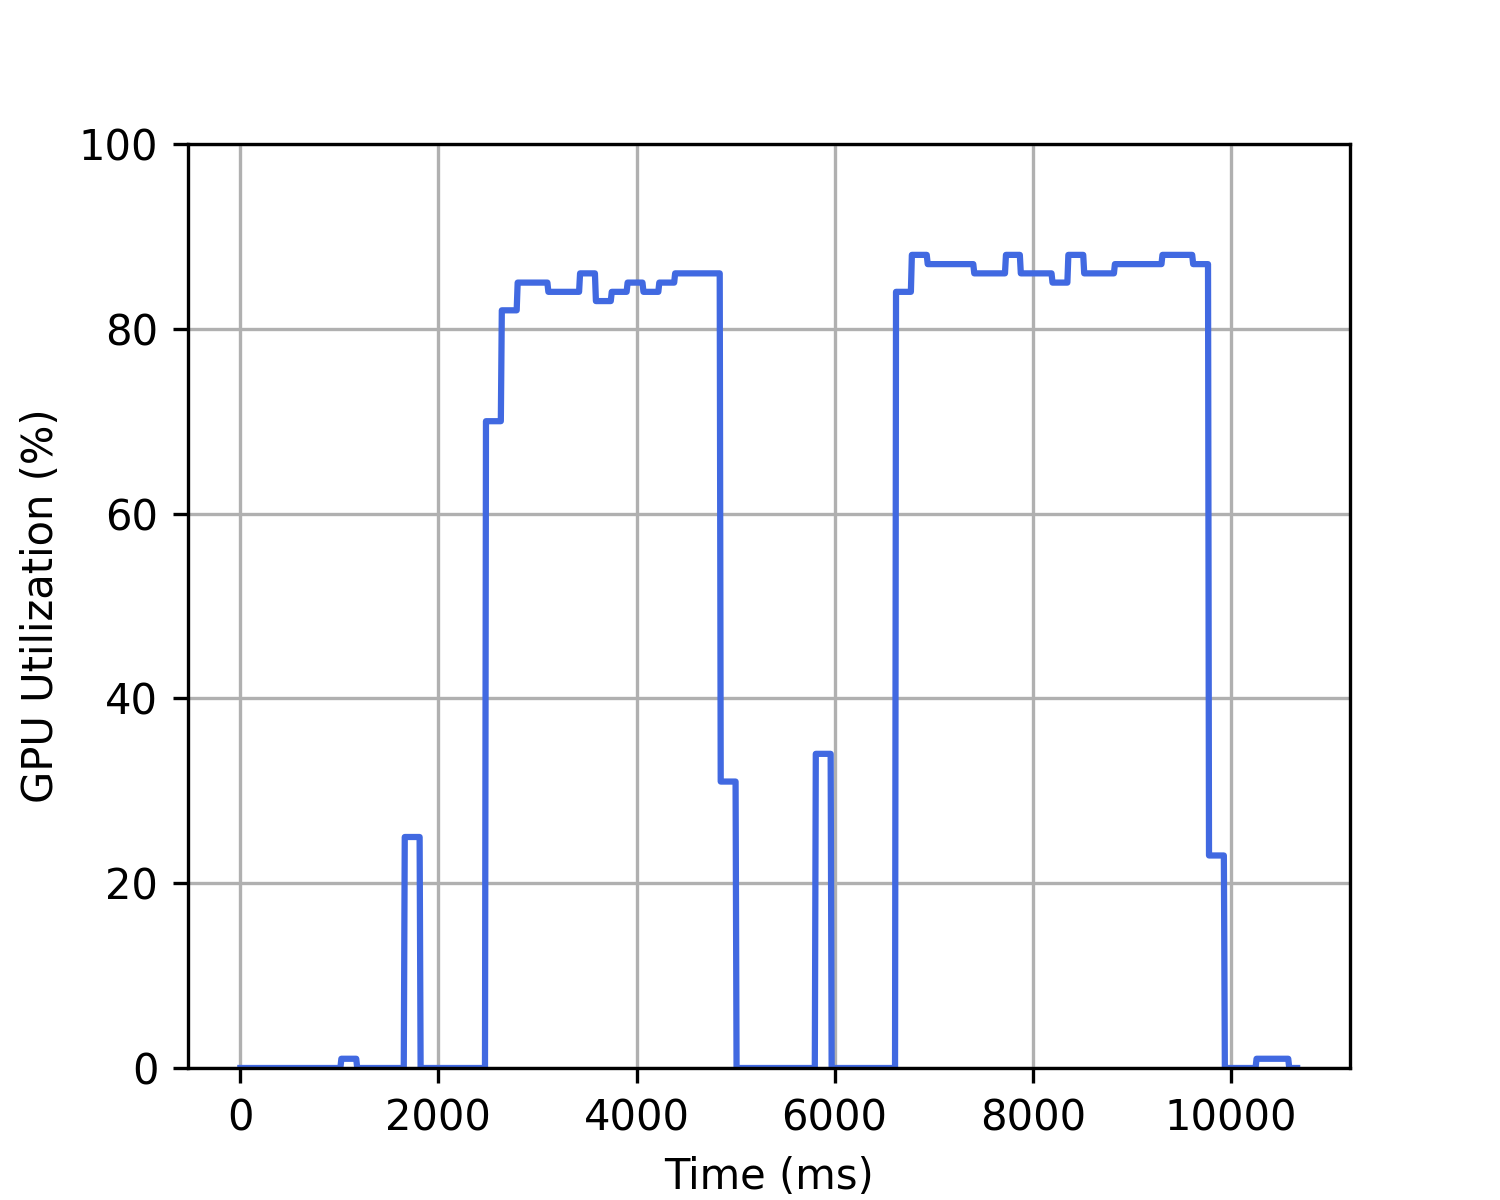
\includegraphics[width=\linewidth]{Chapters/Figures/plots/lmarrow-graph_update_spmv_log_gpu_utilization.png}
        % \label{fig:lmarrow-graph_gpu_utilization}
    \end{subfigure}%
    \begin{subfigure}{0.5\textwidth}
        \centering
        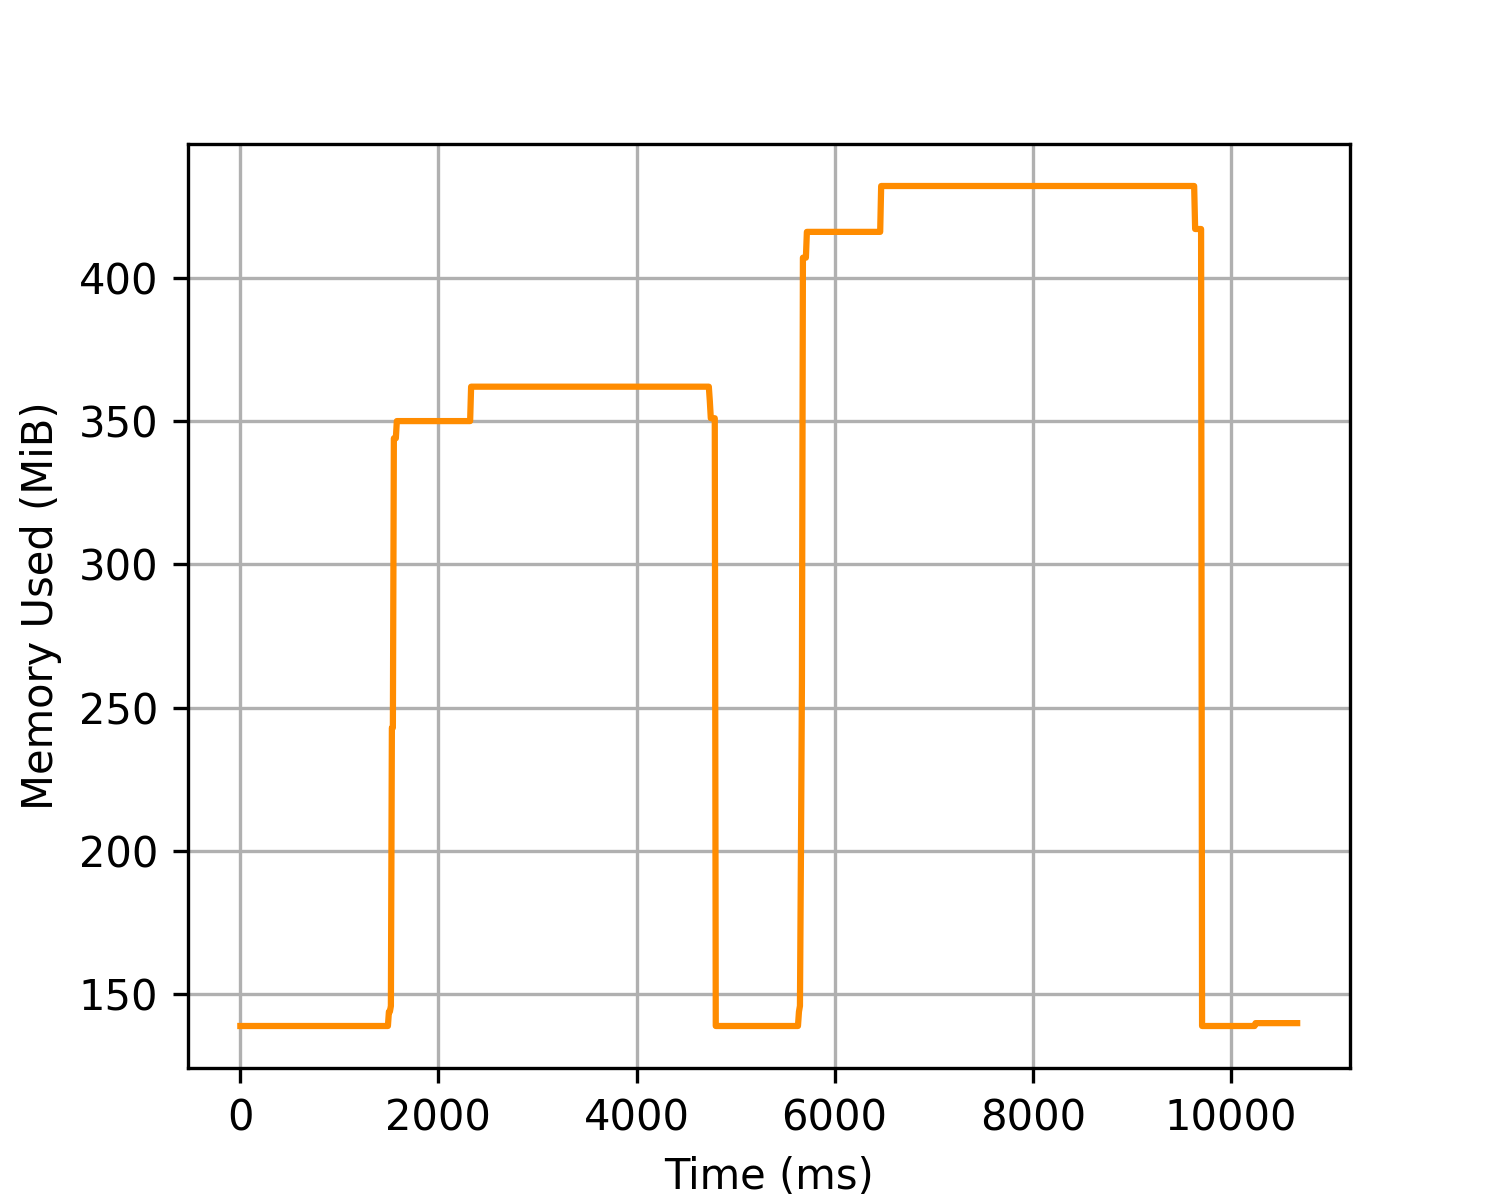
\includegraphics[width=\linewidth]{Chapters/Figures/plots/lmarrow-graph_update_spmv_log_gpu_memory.png}
        % \label{fig:lmarrow-graph_memory_utilization}
    \end{subfigure}%
    \caption{Marrow-Graph GPU utilization.}
    \label{fig:lmarrow-graph_gpu_log}
\end{figure}

\begin{figure}
    \begin{subfigure}{0.5\textwidth}
        \centering
        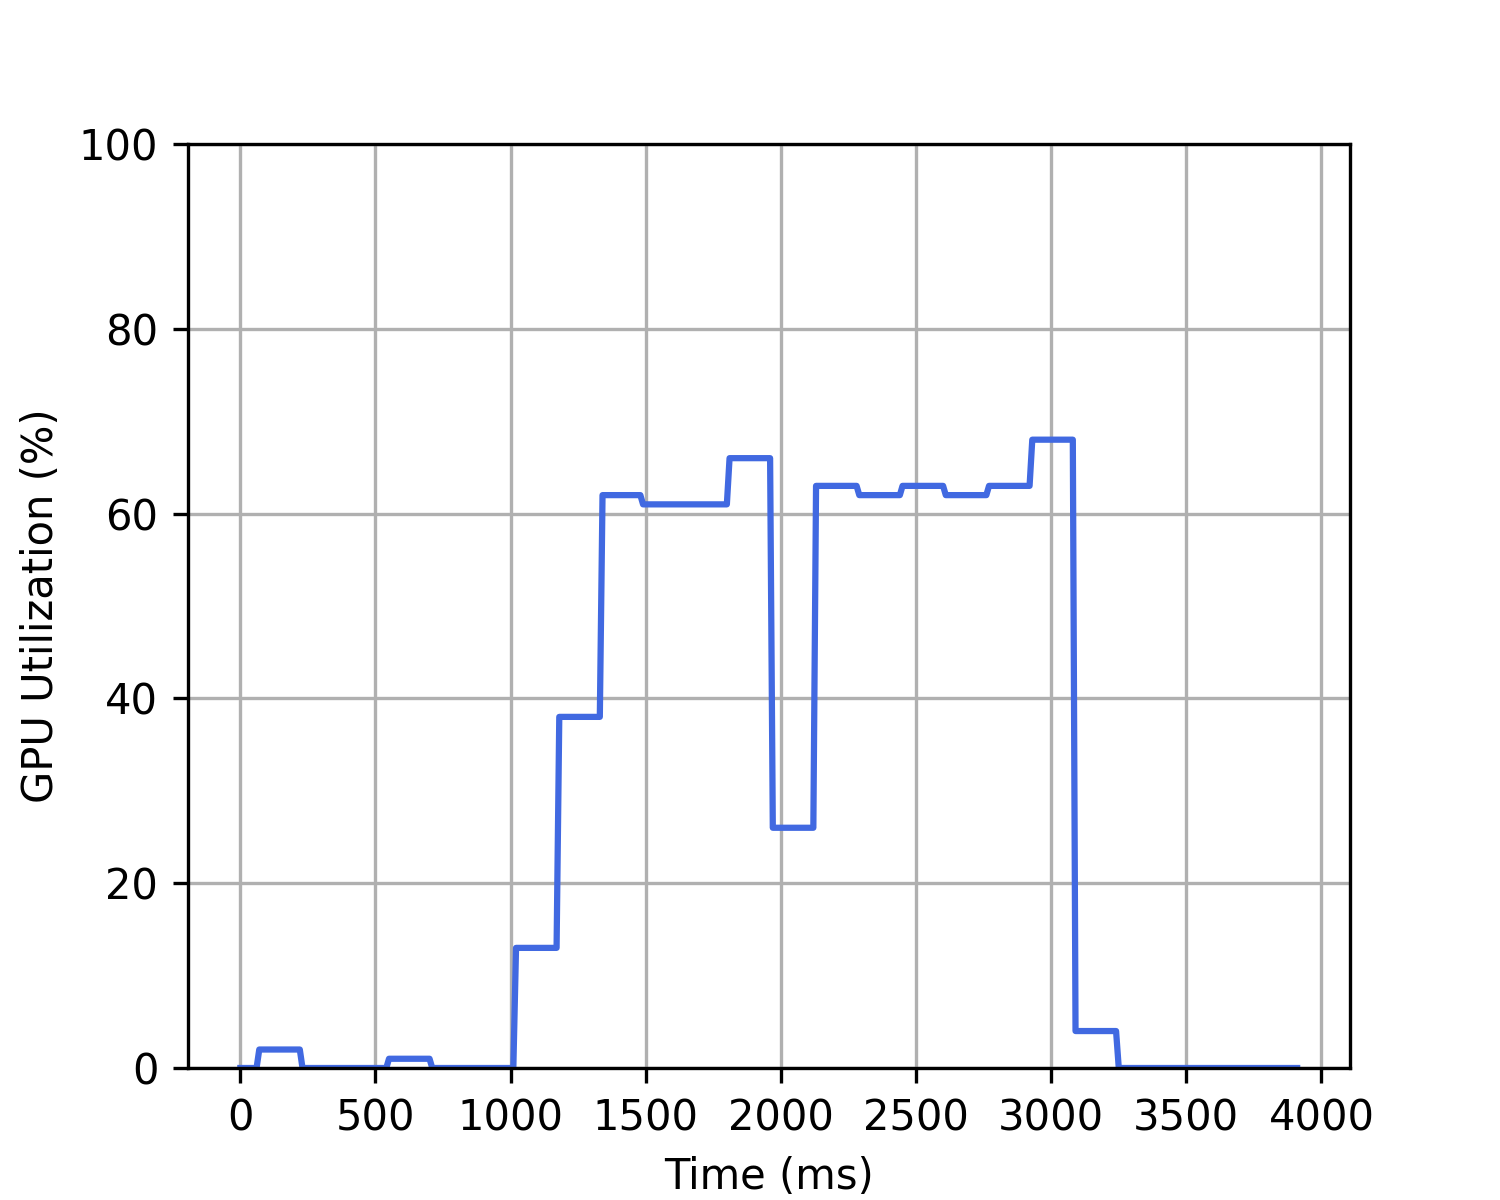
\includegraphics[width=\linewidth]{Chapters/Figures/plots/faimgraph_update_spmv_log_gpu_utilization.png}
        % \label{fig:faimgraph_gpu_utilization}
    \end{subfigure}%
    \begin{subfigure}{0.5\textwidth}
        \centering
        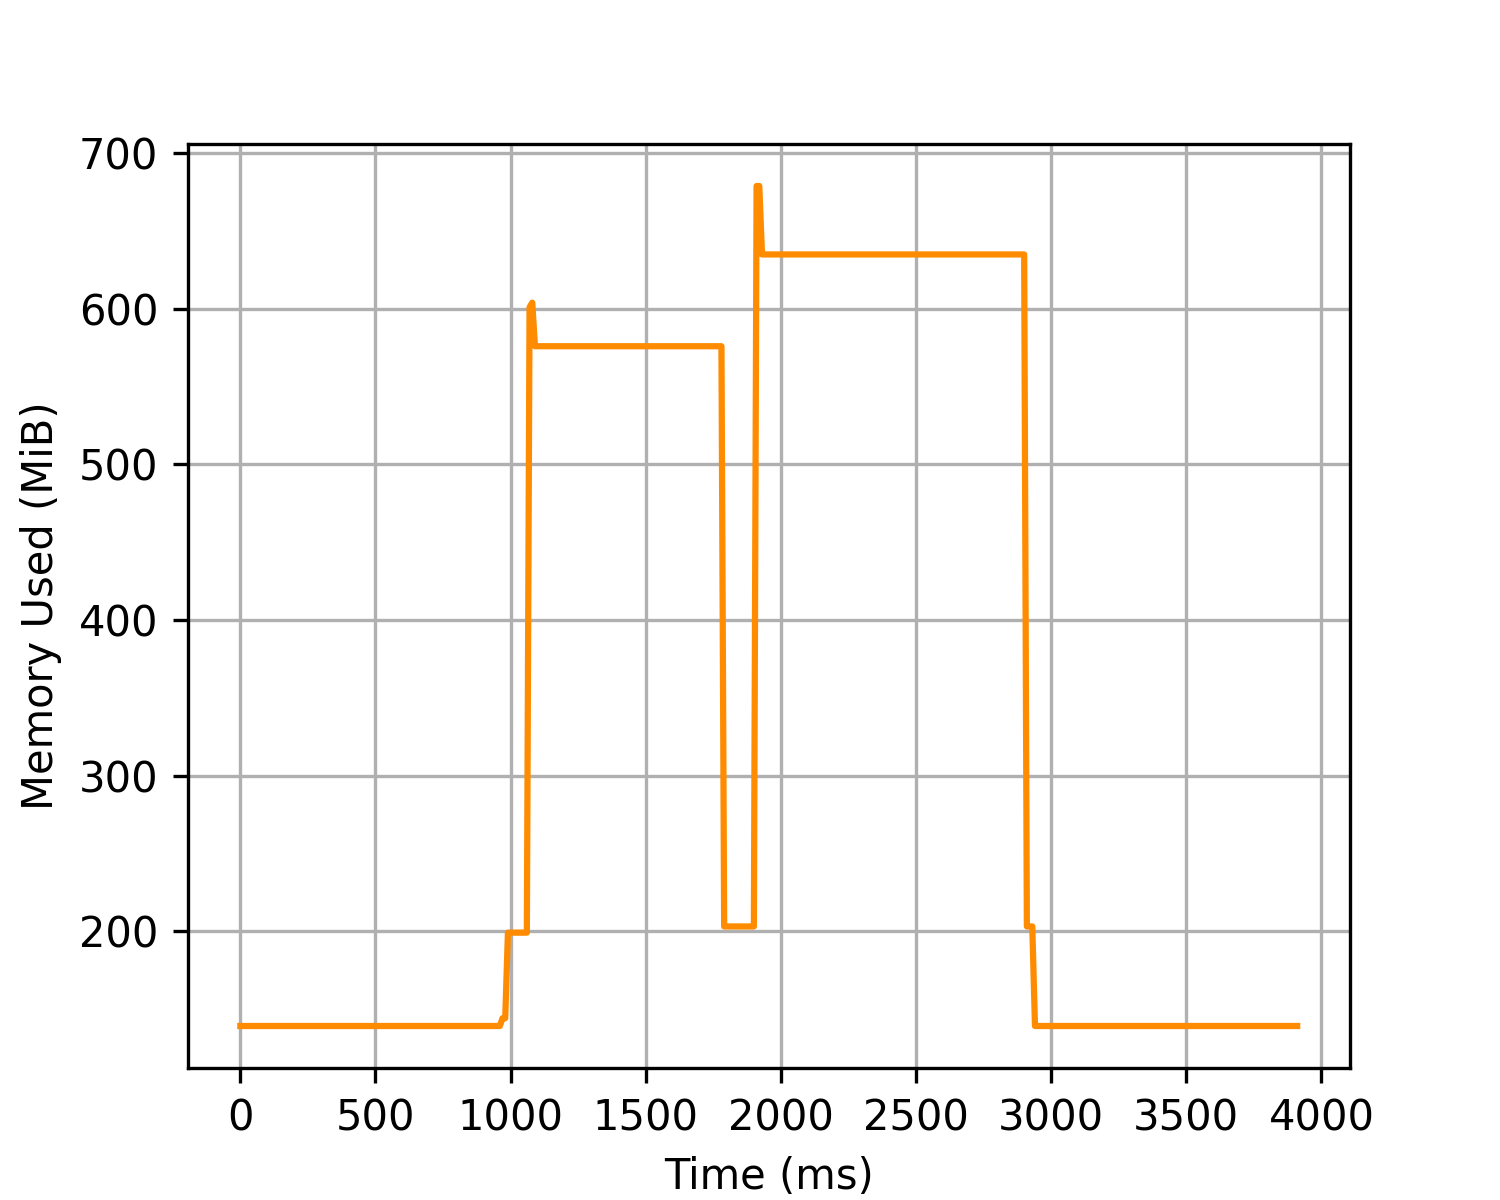
\includegraphics[width=\linewidth]{Chapters/Figures/plots/faimgraph_update_spmv_log_gpu_memory.png}
        % \label{fig:faimgraph_memory_utilization}
    \end{subfigure}%
    \caption{FaimGraph GPU utilization.}
    \label{fig:faimgraph_gpu_log}
\end{figure}

\begin{figure}
    \begin{subfigure}{0.5\textwidth}
        \centering
        \includegraphics[width=\linewidth]{Chapters/Figures/plots/Gunrock_update_spmv_log_gpu_utilization.png}
        % \label{fig:Gunrock_gpu_utilization}
    \end{subfigure}%
    \begin{subfigure}{0.5\textwidth}
        \centering
        \includegraphics[width=\linewidth]{Chapters/Figures/plots/Gunrock_update_spmv_log_gpu_memory.png}
        % \label{fig:Gunrock_memory_utilization}
    \end{subfigure}%
    \caption{Gunrock GPU utilization.}
    \label{fig:Gunrock_gpu_log}
\end{figure}

\subsection{Conclusion}

Returning to our initial questions, we can say that although there is not a general optimal block size, as this depends on the characteristics of the graph being processed, a block size of 8 shows an overall good performance for graphs with average degrees below 16. 



In terms of algorithmic performance, Marrow-Graph has demonstrated superiority over its primary competitor, FaimGraph, in the \gls{SpMV} algorithm, but falls behind in other algorithms such as \gls{BFS} and \gls{TC}. When compared to the static \gls{GPU}-based solutions, Marrow-Graph is often outperformed, although its execution times consistently remain within the same order of magnitude. Despite this, there are instances where Marrow-Graph outperforms Hornet. Notably, Marrow-Graph also showcases remarkable speedups when compared with the only \gls{CPU}-based solution considered, Ligra.
%
Given that there is still a lot of room for performance tweaking, we believe that it is realistic to expect comparable performance to FaimGraph in all benchmarks in the future. 

Regarding graph updates, marrow-graph offers excellent edge insertion rates for small to medium batch sizes. For large batch sizes, the competitors offer better insertion rates given that the batches are inserted in parallel directly on the device. Regardless, marrow-graph achieves very high and consistent insertion rates in the order of $10^5$ and $10^6$ \textit{edges/second}. Additionally, when performing graph updates and analytics interchangeably, Marrow-Graph exhibits excellent performance for small to medium insertion batch sizes, outperforming FaimGraph by large factors.

Finally, in terms of \gls{GPU} utilization, both FaimGraph, Gunrock, and Marrow-Graph show mostly similar results. FaimGraph has some overall higher \gls{VRAM} usage due to its memory manager, and Marrow-Graph exhibits slightly higher \gls{GPU} usage.